% !TEX program = pdflatex
\documentclass[3p,twocolumn,authoryear]{elsarticle}

% ========== 数学与图表宏包 ==========
\usepackage{amsmath,amssymb,amsfonts}
\usepackage{mathtools}
\usepackage{bm}               % bold math symbols
\usepackage{booktabs}          % professional tables
\usepackage{multirow}          % multi-row cells
\usepackage{graphicx}          % figures
\usepackage{subcaption}        % subfigures
\usepackage{algorithm}         % algorithm environment
\usepackage{algorithmic}       % algorithm pseudocode
\usepackage{xcolor}            % colors
\usepackage{enumitem}          % list control
\usepackage{hyperref}          % hyperlinks

% ========== Custom Math Commands ==========
\newcommand{\R}{\mathbb{R}}                              % real numbers
\newcommand{\bF}{\mathbf{F}}                              % feature map
\newcommand{\bq}{\mathbf{q}}                              % query vector
\newcommand{\bu}{\mathbf{u}}                              % unknown query
\newcommand{\bz}{\mathbf{z}}                              % region embedding
\newcommand{\bmu}{\boldsymbol{\mu}}                       % prototype center
\newcommand{\cK}{\mathcal{K}}                             % known class set
\newcommand{\cU}{\mathcal{U}}                             % unknown class set
\newcommand{\tobj}{\tau_{\text{obj}}}                     % no-object threshold
\newcommand{\tabs}{\tau_{\text{abs}}}                     % abstention threshold
\newcommand{\tens}{\tau_{\text{ens}}}                     % ensemble threshold
\DeclareMathOperator*{\argmin}{arg\,min}
\DeclareMathOperator*{\argmax}{arg\,max}

\begin{document}

\begin{frontmatter}
\title{Structured Abstention Segmentation: Native Unknown Representation\\for Open-World Dense Prediction}

\author[addr1]{To be filled}
\address[addr1]{To be filled}

\begin{abstract}
Prevailing medical image segmentation methods are built upon the closed-set assumption,
which compels models to assign every unknown region to some known category,
thereby introducing potentially hazardous misclassifications in clinical practice.
Existing works have largely treated unknown detection as a post-hoc thresholding problem;
however, the capability to \emph{detect} unknown pixels and the capability to
\emph{organize} them into coherent, region-level abstention outputs represent
fundamentally distinct competencies---a distinction that has received insufficient
systematic treatment in the literature.
This paper proposes the \textbf{Structured Abstention Segmentation (SASeg)} framework,
which treats the unknown as a native component of the model's output space:
by introducing dedicated unknown query slots into a Transformer-based region parser,
the unknown competes with known-class queries within the same competitive space to
produce structured abstention outputs, further augmented by a prototype-sphere module
that establishes explicit geometric support boundaries for the known label space.
We design dual evaluation protocols A1/A2 to separately assess
seen-unknown structured abstention and unseen-unknown detection generalization.
Experiments on two multi-organ CT datasets (Synapse and AMOS22) and two natural-image
benchmarks (PASCAL VOC and Cityscapes) reveal:
(1)~native unknown queries are a necessary condition for structured abstention---removing
    them causes unknown F1 to collapse by over 90\%, while post-hoc signals, even when
    retaining pixel-level ranking capability, fail to produce coherent unknown masks;
(2)~high detection ranking performance in A2 (AUROC$>$0.97) does not imply usable
    structured abstention outputs, and region-level analysis reveals that candidate purity
    is the core bottleneck for unseen-unknown structuring;
(3)~both phenomena hold consistently on PASCAL VOC and Cityscapes, confirming that they
    are not artifacts of medical CT imaging but general properties of structured abstention
    in dense segmentation.
The contribution of this work lies not in proposing a detector that comprehensively
outperforms all baselines, but in establishing the problem formulation and evaluation
framework for structured abstention, verifying the necessity of native unknown
representation, and characterizing the fundamental barrier to translating detection
into structuring as a domain-general challenge in open-world dense segmentation.
\end{abstract}

\begin{keyword}
semantic segmentation \sep open-world recognition \sep structured abstention \sep prototype sphere \sep region parsing
\end{keyword}
\end{frontmatter}


% ============================================================
%  SASeg — Introduction & Related Work
%  Target journal: Knowledge-Based Systems
% ============================================================

\section{Introduction}
\label{sec:intro}

% ----------------------------------------------------------------
%  Paragraph 1: Problem significance — closed-set assumption fails in clinical deployment
% ----------------------------------------------------------------

Deep-learning-based segmentation models have achieved remarkable performance across
a wide range of medical imaging tasks, including organ segmentation in CT images
and lesion segmentation in MRI images
\cite{zhao2023efficientmulti,zeineldin2022multimodalcnn}.
Nevertheless, nearly all prevailing models are built upon the \emph{closed-set assumption}:
every pixel in the input image is presumed to belong to one of the anatomical categories
defined during training.
In real clinical scenarios, this assumption is frequently violated.
Images may contain anatomical structures never annotated in the training set---such as
rare lesions, unlabeled organs, or vascular variants---and may further exhibit
distribution shifts arising from different scanning devices, contrast protocols, or
patient populations.
Under the closed-set assumption, the model is forced to assign each pixel to the most
similar known category, thereby producing \emph{high-confidence yet silently erroneous}
predictions in unknown regions.
This failure mode is particularly dangerous in safety-critical medical applications,
where downstream clinical decisions depend directly on the trustworthiness of
segmentation outputs
\cite{kompa2021secondopinion,li2025evaluationuncertainty,miranda2024exploringtransformer}.
While especially acute in clinical settings, the closed-set limitation is not unique
to medical imaging: any dense segmentation system deployed in an open world---whether
for natural scene understanding or autonomous driving---faces the same structural
challenge of encountering categories not present during training.

% ----------------------------------------------------------------
%  Paragraph 2: Limitations of existing methods — from "can we detect" to "can we structure"
% ----------------------------------------------------------------

Existing methods for handling unknown regions in segmentation can be broadly
categorized into two families.

The first family employs \emph{post-hoc risk scores}:
after a standard closed-set model generates per-pixel predictions, auxiliary signals
are computed---such as maximum softmax probability (MSP), energy scores,
or Monte Carlo Dropout variance---to estimate pixel-level uncertainty,
which is then thresholded to delineate unknown regions.
The second family appends an \emph{auxiliary unknown branch} outside the standard
encoder–decoder (typically a binary classification head mounted on a U-Net backbone)
to predict whether each pixel is unknown.
Representative methods of the former family include MSP, Energy, and MC-Dropout
\cite{hendrycks2017baselinedetecting,liu2020energyout,gal2016dropoutbayesian},
with related outlier-aware segmentation explorations in dense prediction settings
\cite{grcic2023advantagesmask}.
While both families demonstrate certain anomaly detection capabilities,
they share a fundamental limitation:
\textbf{the unknown is treated as a by-product of the prediction pipeline
rather than a native constituent of the output space.}
Post-hoc scores reduce the problem to pixel-level ranking and cannot yield coherent
region-level masks; auxiliary unknown branches introduce a separate prediction pathway
that does not compete within the same spatial budget as known-class predictions.
Moreover, both families are prone to systematic false positives at anatomical boundaries---
a consequence of partial-volume effects that naturally elevate uncertainty at organ
boundaries, a pervasive issue in multi-organ CT segmentation
\cite{li2020superpixelguided,yeung2021incorporatingboundary,mukul2020uncertaintygraph,hassan2024udbrnetnovel}.

%% [Figure suggestion — Fig. 1: Motivation comparison]
%% Recommended placement after this paragraph.
%% Design:
%%   Left (a): "Post-hoc uncertainty" — show MSP/Energy thresholding results on a CT slice,
%%             with high-uncertainty pixels scattered and unable to form coherent regions,
%%             with organ boundaries largely mislabeled as unknown.
%%   Right (b): "Native unknown slot" — the same slice with our method's output,
%%             where the unknown region is a spatially coherent mask competing with
%%             known-class masks within the same region parser.
%% Source: Select from the T2 experiment M=2 vs M=0 visualization,
%%         or from a representative Synapse slice prediction result.
%% \begin{figure}[t]
%%   \centering
%%   \includegraphics[width=\linewidth]{fig/motivation_comparison.pdf}
%%   \caption{Comparison of post-hoc uncertainty thresholding versus native structured abstention.
%%   (a) Post-hoc methods produce scattered high-risk pixels that cannot form coherent unknown regions.
%%   (b) Our native unknown slots compete within the same region parsing framework as known queries,
%%   yielding structured abstention masks.}
%%   \label{fig:motivation}
%% \end{figure}

% ----------------------------------------------------------------
%  Paragraph 3: Core insight + overview of proposed approach
% ----------------------------------------------------------------

A central observation of this paper is:
\textbf{the ability to \emph{detect} unknown pixels is fundamentally distinct from
the ability to \emph{structure} them into coherent abstention regions.}
Detection concerns whether a scoring function can rank unknown pixels above known ones;
structuring concerns whether the model can organize those pixels into spatially coherent,
region-level masks that are directly usable in clinical workflows.
We argue that these are two essentially different capabilities, and conflating them
under a single evaluation metric obscures critical failure modes.

Motivated by the above observation, we formalize the concept of \emph{structured abstention}
in medical image segmentation and propose a systematic research framework.
The framework comprises three components.

\textbf{First}, we introduce two complementary evaluation protocols---
\textbf{A1} (seen-unknown structuring) and
\textbf{A2} (unseen-unknown detection generalization)---that
explicitly decouple the assessment of structuring capability from detection capability.

\textbf{Second}, we propose a \emph{region parsing architecture with native unknown slots}:
learnable unknown queries jointly participate in parsing alongside known anatomy queries
within the same Transformer-based region competition framework,
so that unknown regions emerge as first-class components of the output rather than
being appended as post-hoc additions.
Furthermore, a \emph{prototype-sphere support module} maintains explicit geometric support
boundaries for each known class, providing a knowledge-driven mechanism to determine
whether a given region falls within the support domain of any known anatomical category.

\textbf{Third}, we design a multi-signal decision framework that fuses geometric support
scores and mask-level uncertainty, acknowledging that different unknown regimes are
dominated by different leading signals.

% ----------------------------------------------------------------
%  Paragraph 4: Preview of key findings
% ----------------------------------------------------------------

Experiments on the Synapse multi-organ CT dataset and the AMOS22 dataset, further
validated on PASCAL VOC and Cityscapes, yield several findings with important
implications for open-world dense segmentation research:

\begin{itemize}
  \item \textbf{The $M=0$ ablation}---removing all native unknown slots---
  causes unknown F1 on Synapse to collapse from 0.721--0.728 (depending on the
  unknown signal selection) to 0.008--0.070, and on AMOS22 from 0.839 to 0.045,
  while known-class mIoU is almost unaffected.
  This demonstrates that native unknown slots are a \emph{necessary condition}
  for structured abstention in the seen-unknown (A1) setting, and that post-hoc
  signals---even when retaining strong pixel-level ranking capability---cannot
  substitute for explicit allocation within the native output space.

  \item In the unseen-unknown (A2) setting, ensemble detection scores achieve
  AUROC$>$0.97 on both datasets; however, pixel-level unknown F1 remains near zero.
  This \emph{detection--structuring gap} reveals that high-quality detection signals
  do not automatically translate into usable structured abstention outputs.

  \item Region-level analysis further demonstrates that the bottleneck in A2 lies not
  in the final decision threshold but in \emph{candidate purity}: the coarse
  responses produced by unknown slots rarely achieve IoU$\geq$0.10 with ground-truth
  unknown regions, indicating that the generation of reliable unknown region candidates
  itself remains an open challenge.

  \item Cross-domain experiments on PASCAL VOC and Cityscapes confirm that both the
  $M{=}0$ collapse and the detection--structuring gap hold consistently in natural-image
  semantic segmentation tasks with markedly different visual characteristics from medical
  CT, establishing that these phenomena are general properties of structured abstention
  in dense segmentation rather than domain-specific artifacts.
\end{itemize}

% ----------------------------------------------------------------
%  Paragraph 5: Summary of contributions
% ----------------------------------------------------------------

In summary, this paper makes the following contributions:

\begin{enumerate}
  \item We formalize the concept of \textbf{structured abstention} in dense segmentation
  and introduce two evaluation protocols, A1 (seen-unknown structuring) and A2
  (unseen-unknown detection), that for the first time explicitly decouple the assessment
  of unknown structuring capability from detection capability.

  \item We propose a \textbf{native unknown-slot region parser} and a prototype-sphere
  support module. Through $M{=}0$ ablation experiments on two independent medical CT
  datasets (Synapse and AMOS22) and two natural-image benchmarks (VOC and Cityscapes),
  we demonstrate that a native unknown output space is a necessary condition for
  structured abstention in the A1 setting across diverse visual domains.

  \item We reveal that \textbf{detection and structuring are fundamentally distinct
  sub-problems}: even with high-quality detection signals (AUROC$>$0.97),
  pixel-level structuring can completely fail.
  Through pixel-level retrieval analysis and region-level candidate purity analysis,
  we identify candidate purity---rather than detection scores or decision thresholds---
  as the dominant bottleneck for unseen-unknown structuring.
  Cross-domain validation on VOC and Cityscapes further confirms that the
  detection--structuring gap is a general property of dense segmentation, not an
  artifact of medical imaging.
\end{enumerate}


% ============================================================
\section{Related Work}
\label{sec:related}
% ============================================================

We review four lines of research most closely related to structured abstention
in medical image segmentation.
This section addresses the first two;
the latter two (query-based segmentation architectures and prototype-based methods)
are discussed in Section~\ref{sec:rw-query} and Section~\ref{sec:rw-proto},
respectively.

% -----------------------------------------------------------
\subsection{Open-Set Recognition and Out-of-Distribution Detection}
\label{sec:rw-osr}
% -----------------------------------------------------------

Open-Set Recognition (OSR) aims to classify inputs from known categories while
rejecting inputs belonging to categories unseen during training.
Early work modeled the problem as thresholding calibrated confidence scores.
Bendale and Boult proposed OpenMax, which, grounded in extreme value theory,
replaces the closed-set softmax layer with an open-set scoring function, enabling
the network to output explicit ``unknown'' probabilities~\cite{bendale2016towardsopen}.
Subsequent works explored various rejection criteria.
Chen et al.\ proposed Adversarial Reciprocal Point Learning (ARPL), which jointly
maintains prototypes for known classes and for the open space to separate the
two~\cite{chen2022adversarialreciprocal}.
Zhou et al.\ introduced learnable placeholders to reserve representational space for
potential unknown classes~\cite{zhou2021learningplaceholders}.

In parallel, Out-of-Distribution (OoD) detection focuses on distinguishing in-distribution
inputs from those originating from different data sources.
Hendrycks and Gimpel established the widely used MSP baseline, employing the maximum
softmax probability as a confidence indicator~\cite{hendrycks2017baselinedetecting}.
Liu et al.\ proposed the energy score, demonstrating that the log-sum-exp of logits
provides a theoretically grounded and empirically superior alternative to
MSP~\cite{liu2020energyout}.
More recent work further leverages virtual outlier synthesis---generating pseudo-OoD
features during training---as well as vision-language priors for open-vocabulary OoD
detection~\cite{he2022ronfreliable,ming2022delvingout}.
Yang et al.\ provided a comprehensive survey that unifies OoD detection taxonomies
across classification, detection, and segmentation tasks~\cite{yang2024generalizedout}.

%% [Figure suggestion — Fig. 2: Task hierarchy comparison]
%% Recommended placement here or before the next paragraph.
%% A three-level comparison figure:
%%   (a) Image-level OSR  → one accept/reject decision per image
%%   (b) Object-level open-set detection → known/unknown at bounding-box level
%%   (c) Pixel-level structured abstention (ours) → coherent unknown mask at pixel level
%% Purpose: allow readers to immediately see the level difference between this work
%%          and existing approaches.
%% \begin{figure}[t]
%%   \centering
%%   \includegraphics[width=0.85\linewidth]{fig/task_hierarchy.pdf}
%%   \caption{Three granularity levels of unknown rejection.
%%   Existing methods operate at the image level~(a) or object level~(b).
%%   This paper addresses pixel-level structured abstention~(c),
%%   which requires generating coherent region masks for unknown content
%%   rather than merely per-pixel scores.}
%%   \label{fig:task-hierarchy}
%% \end{figure}

A growing body of work extends OSR and OoD detection from image-level classification
to \emph{object-level} detection.
Open-world object detection methods, such as OW-DETR, train an explicit ``unknown''
query alongside known-class queries, enabling the detector to localize objects from
novel categories at inference time~\cite{gupta2021owdetr}.
Subsequent works further extend this direction from the perspectives of unknown object
recognition and open-vocabulary supervision~\cite{fang2023unsupervisedrecognition,wang2024ovdquo}.

Despite significant progress at the image and object levels,
\textbf{the extension to pixel-level structured abstention in dense segmentation
remains largely unexplored.}
The key distinction is that segmentation requires not only detection
(i.e., ranking unknown pixels above known ones in a score)
but also \emph{structuring}: organizing those pixels into spatially coherent region masks.
Existing OSR/OoD methods produce per-pixel or per-instance anomaly scores,
but do not address whether such scores can be assembled into usable segmentation outputs.
This paper bridges this gap by formalizing structured abstention as a first-class objective
and providing an evaluation protocol that explicitly separates detection from structuring.

\begin{figure}[htbp]
    \centering
    \includegraphics[width=0.95\linewidth]{saseg_hierarchy_diagram.drawio.png}
    \caption{Comparison of open-world recognition paradigms. Existing methods predominantly focus on image-level anomaly scoring (e.g., OSR) or object-level bounding box detection, which lack spatial coherence for dense prediction tasks. We identify a critical \textit{detection-structuring gap}---the fundamental limitation where even high-quality pixel-level detection scores cannot be trivially thresholded to form clinically usable, structured regions. Our proposed Structured Abstention Segmentation (SASeg) addresses this by elevating unknown regions to first-class structural outputs at the pixel level.}
    \label{fig:paradigm_hierarchy}
\end{figure}


% -----------------------------------------------------------
\subsection{Anomaly Detection and Out-of-Distribution Detection in Medical Imaging}
\label{sec:rw-med-ood}
% -----------------------------------------------------------

The safety-critical nature of medical imaging has given rise to a dedicated line of
research focused on detecting anomalous or out-of-distribution content in clinical data.
The Medical Out-of-Distribution (MOOD) challenge established a benchmark in which
models are trained solely on normal brain or abdominal scans and evaluated at inference
time on their ability to localize anomalies (such as lesions, artifacts, and synthetic
degradations)~\cite{zimmerer2022mood2020}.
Competing approaches explored diverse anomaly scoring paradigms,
including reconstruction-based methods---flagging regions with high reconstruction error
under autoencoders trained on normal data;
self-supervised contrastive objectives---learning compact representations of normal
anatomy and detecting deviations at test time;
and feature-matching methods---comparing test-time activations against an in-distribution
feature memory bank.
Representative medical anomaly localization works include autoencoder reconstruction-based
approaches, three-dimensional spatial erasing strategies, and recent masked autoencoder
based methods~\cite{baur2021autoencodersunsupervised,bengs2021threedimensional,rashmi2024anoswinmae}.

Uncertainty estimation provides a complementary perspective for medical OoD detection.
Monte Carlo Dropout and deep ensembles remain the most widely adopted approaches,
as they can be applied as plug-and-play additions to existing segmentation architectures
with minimal modification~\cite{lambert2022trustworthyclinical,musah2025towardstrustworthy}.
By executing multiple stochastic forward passes (or aggregating predictions from multiple
independently trained models), these methods produce voxel-level variance maps as
proxies for epistemic uncertainty.
Lambert et al.\ provided a comprehensive survey of uncertainty quantification in
deep learning-based medical image segmentation, cataloguing over 200 methods and
noting that most evaluation protocols remain at the pixel level, without considering
structure-level evaluation aligned with clinical concerns~\cite{lambert2022trustworthyclinical}.

Published in Knowledge-Based Systems, Wang et al.\ proposed UG-Net, which learns from
uncertainty in an end-to-end manner by feeding coarse-grained uncertainty maps into a
refinement module, demonstrating that uncertainty can be exploited as an internal
architectural signal rather than merely a post-hoc output~\cite{wang2022uncertaintyguided}.
This idea is conceptually aligned with our approach of embedding the unknown into the
native output space; however, UG-Net still operates within a closed-set label space
and does not explicitly model unknown categories.

More recently, several works have examined the reliability of segmentation models
from the perspective of selective prediction and abstention.
Under this paradigm, the model is permitted to ``abstain'' on inputs (or regions)
where confidence is insufficient, trading coverage for accuracy.
While selective prediction has been extensively studied in the classification
setting---with representative works including SelectiveNet and survey discussions
on the safe deployment of medical machine
learning~\cite{geifman2019selectivenetdeep,kompa2021secondopinion}---its application
to dense segmentation---where the unit of abstention is not a single image but a
\emph{structured spatial region}---has received comparatively limited attention.
From the dense prediction perspective, methods such as MaskFormer have demonstrated
that semantic segmentation need not be reduced to per-pixel classification but can
instead be framed as mask-level prediction, and recent work on outlier-aware
segmentation further shows that pixel-level anomaly scoring and spatially coherent
mask-level unknown representation are not
equivalent~\cite{cheng2021perpixel,grcic2023advantagesmask}.

Despite the above advances, existing medical OoD detection methods share two important
limitations that this paper aims to address.

\textbf{First, existing methods output unstructured anomaly score maps rather than
structured segmentation outputs.}
Per-pixel uncertainty or reconstruction-error heatmaps still require thresholding and
post-processing to produce usable masks, and this thresholding step is rarely studied
systematically.
As we show in this paper, high-quality pixel-level ranking (e.g., AUROC$>$0.97)
does \emph{not} guarantee that a usable structured mask can be derived from it---
a phenomenon we term the \emph{detection--structuring gap}.

\textbf{Second, existing methods do not distinguish between different unknown regimes.}
Our experiments reveal that seen unknowns (anatomical structures present in training
cases but excluded from the known label set) and unseen unknowns (structures completely
absent during training) exhibit qualitatively different failure modes:
the former is primarily a structuring challenge, while the latter additionally involves
the challenge of detection generalization.
Handling both regimes under a single evaluation protocol risks conflating these two
distinct difficulties, thereby obscuring important failure modes.

Our framework addresses both limitations simultaneously by introducing a native
unknown output space (rather than post-hoc scoring) and dual evaluation protocols
A1/A2 (assessing structuring and detection separately).
Although the discussion above is situated in the medical imaging context,
these limitations apply equally to any dense segmentation setting where unknown
categories may appear at inference time.

%% [Figure suggestion — summary positioning table]
%% A comparison table can be placed after the end of Related Work (i.e., after §2.4),
%% contrasting research paradigms across four dimensions:
%% "Detection," "Structuring," "Medical," and "Granularity."
%% This allows reviewers to immediately see the unique positioning of this paper.
%% \begin{table}[t]
%%   \centering
%%   \caption{Positioning of this paper relative to existing research paradigms.
%%   ``Detection'' = scoring/ranking capability; ``Structuring'' = structured region output;
%%   ``Medical'' = targeting medical imaging.}
%%   \label{tab:rw-positioning}
%%   \small
%%   \begin{tabular}{lcccl}
%%     \toprule
%%     \textbf{Paradigm} & \textbf{Detection} & \textbf{Structuring} & \textbf{Medical} & \textbf{Granularity} \\
%%     \midrule
%%     OSR (OpenMax, ARPL)          & \cmark & \xmark & \xmark & Image \\
%%     OoD Detection (MSP, Energy)  & \cmark & \xmark & Partial & Pixel score \\
%%     Open-set object detection    & \cmark & Partial & \xmark & BBox \\
%%     Medical anomaly detection    & \cmark & \xmark & \cmark & Pixel score \\
%%     Uncertainty segmentation     & \cmark & \xmark & \cmark & Pixel score \\
%%     \textbf{This paper (SASeg)}  & \cmark & \cmark & \cmark & Region mask \\
%%     \bottomrule
%%   \end{tabular}
%% \end{table}


% -----------------------------------------------------------
\subsection{Query-Based Segmentation Architectures}
\label{sec:rw-query}

In recent years, semantic and instance segmentation have progressively shifted from
the traditional per-pixel classification paradigm toward \emph{mask-level parsing}.
MaskFormer explicitly argues that semantic segmentation need not be equivalent to
classifying each pixel independently; instead, a set of learnable queries can predict
a set of masks and their semantic labels, reformulating dense prediction as a set
prediction problem~\cite{cheng2021perpixel}.
Building on this, FastInst demonstrates the simplicity and efficiency of query-based
mask parsing in real-time segmentation, while Mask DINO further unifies the Transformer
decoding framework for detection and segmentation tasks, establishing query-driven
region parsing as an important technical direction in visual
segmentation~\cite{he2023fastinstsimple,li2022maskdino}.
Recent work has also begun discussing the adaptability of queries themselves in
continual segmentation and open-environment settings, indicating that query design is
not a fixed engineering detail but directly affects how models parse novel categories
and novel scenes~\cite{zhu2025rethinkingquery}.

These works provide a key starting point for this paper:
\textbf{query-based architectures are naturally suited for modeling region-level outputs.}
However, the output space of existing methods remains closed-set by default:
queries are responsible for ``which known class'' or ``which instance,''
not for ``how to reserve a native output slot for the unknown.''
In other words, existing query-based segmentation methods have addressed the question
of \emph{how to parse regions}, but have not explicitly answered \emph{how to preserve
first-class status for unknown regions within the same parsing space.}
This paper does not reinvent the query parser; rather, it introduces native unknown
slots into this mature framework, so that unknown regions no longer depend on
post-hoc scores or external binary branches, but instead emerge jointly with known
queries through the same Transformer region competition mechanism.

\subsection{Prototype-Based Visual Recognition Methods}
\label{sec:rw-proto}

Parallel to query-based segmentation, another line of research employs prototypes,
prototype-spheres, or open-space representations to characterize the feature support
domain of known classes.
In open-set recognition, OpenMax corrects the overconfidence of closed-set softmax
by modeling tail distributions, while subsequent placeholder learning and ARPL further
model the ``unknown'' in terms of positional relationships relative to known-class
prototypes: the former reserves representational slots for potential unknown categories,
while the latter explicitly widens the gap between the known space and the open space
via reciprocal points and adversarial
learning~\cite{bendale2016towardsopen,zhou2021learningplaceholders,chen2022adversarialreciprocal}.
The common thread across these methods is that they do not rely solely on a single
confidence score, but instead attempt to establish some geometric support boundary
for known classes in the feature space.

The prototype-sphere support module in this paper shares the geometric motivation of
this line of research, but differs in how it operates.
Existing prototype-based OSR methods mostly serve \emph{class matching or sample
rejection}: determining which known class an input is closest to, or whether it should
be judged as an open-space sample.
In this paper, the prototype-sphere does not directly assume the class parsing function
of the region parser; instead, it serves as a \emph{region support arbiter}: after the
queries have already generated candidate masks, it determines whether the corresponding
region embedding is still supported by any known label space.
Accordingly, we borrow the geometric intuition of prototype-based recognition but
repurpose it from ``class prototype matching'' to ``support domain boundary judgment,''
enabling it to work synergistically with the query-based region parser toward the
shared goal of pixel-level open-world structured abstention.




% ======================================================================
%  §3  Problem Formulation
% ======================================================================
\section{Problem Formulation}\label{sec:problem}

\subsection{Structured Abstention Segmentation}\label{sec:problem:sa}

Let the input image be $\mathbf{X} \in \R^{H \times W \times C}$ and the known class
label set be $\cK = \{1, \ldots, K\}$.
Under the closed-set segmentation paradigm, the model is required to output a label
$y_p \in \cK \cup \{0\}$ for each pixel $p$ (where $0$ denotes background), implicitly
assuming that all foreground pixels can be accurately described by some class in $\cK$.
In practice, however, images inevitably contain categories never annotated during
training---in medical CT, these may be rare lesions, unlabeled organs, or vascular
variants; in natural-image segmentation, they may be novel object classes or uncommon
scene elements---collectively referred to as \textbf{unknown regions}.
Closed-set models are forced to assign such regions to the most similar known class,
producing erroneous predictions that carry potential harm in safety-critical applications.

This paper formalizes the above problem as \textbf{Structured Abstention Segmentation (SASeg)}:
the model's output space is extended from $\cK \cup \{0\}$ to
$\cK \cup \{0, \texttt{unknown}\}$,
where $\texttt{unknown}$ is not a pixel set delineated post-hoc by an uncertainty
threshold, but rather a native component of the model's output space---produced by
a dedicated query slot that competes with known-class queries during the region-level
parsing process.
The key distinction of this formulation is:
\begin{itemize}[nosep]
  \item Post-hoc methods (e.g., MSP thresholding, energy scores) merely apply a
        secondary judgment to the confidence of existing predictions and cannot guarantee
        spatial coherence of the unknown region;
  \item In our framework, unknown queries compete with known-class queries for attention
        resources within the same Transformer decoder, thereby producing structured
        abstention outputs at the region level.
\end{itemize}

\subsection{Dual-Protocol Evaluation Framework}\label{sec:problem:protocol}

We further argue that unknown segmentation involves two \textbf{fundamentally distinct}
capabilities at the evaluation level, which should not be conflated under a single
metric system. To this end, we design the following dual protocol:

\paragraph{Protocol A1 (Seen-Unknown Structured Abstention)}
The training set contains annotations for $\cK$ as well as annotations for a set of
seen unknown classes $\cU_{\text{seen}}$.
The unknown regions in the test set are of the same classes as those in the training set.
The primary metrics are unknown F1, IoU, Precision, and Recall,
measuring whether the model can \textbf{structure} seen unknown regions into coherent
segmentation masks.

\paragraph{Protocol A2 (Unseen-Unknown Detection Generalization)}
The training set is the same as A1, but the test set contains unknown classes
$\cU_{\text{unseen}}$ that were \textbf{never seen} during training
($\cU_{\text{seen}} \cap \cU_{\text{unseen}} = \emptyset$).
Because the model has no prior knowledge of $\cU_{\text{unseen}}$,
pixel-level F1/IoU would be severely distorted by extreme class imbalance;
the primary metrics are therefore threshold-independent detection measures:
AUROC, AUPR, and FPR@TPR95, assessing whether the model can assign higher
anomaly scores to unseen unknown pixels relative to known-class pixels.

The fundamental distinction between the two protocols lies in the type of capability
being examined:
A1 examines \textbf{structuring capability}---whether unknowns can be organized into
spatially coherent regions;
A2 examines \textbf{detection generalization capability}---whether effective ranking
signals can be produced for unseen unknowns.
Subsequent experiments (Section~\ref{sec:exp}) will demonstrate that these two
capabilities are dominated by different signals and exhibit markedly different
performance profiles, validating the necessity of the dual-protocol split.


% ======================================================================
%  §4  Methodology
% ======================================================================
\section{Methodology}\label{sec:method}

This section details the proposed structured abstention segmentation framework.
The overall pipeline, illustrated in Figure~\ref{fig:architecture},
consists of four cascaded modules:
(1)~Encoder,
(2)~Pixel Decoder,
(3)~Region Parser, and
(4)~Support Module.

\begin{figure*}[htbp]
    \centering
    \includegraphics[width=0.95\textwidth]{saseg_architecture_diagram.drawio.png}
    \caption{Overall architecture of the proposed SASeg framework. The input image is processed by an encoder and a pixel decoder to extract a dense feature map $F$. The region parser utilizes a Transformer decoder to parse learnable queries (known/unknown/background/no-object) into corresponding mask logit maps. The support module determines the knownness of each region based on prototype-sphere geometry, ultimately producing pixel-wise segmentation results that include the unknown label.}
    \label{fig:architecture}
\end{figure*}

% ---------- 4.1 Overall Architecture Overview ----------
\subsection{Overall Architecture Overview}\label{sec:method:overview}

Given an input image $\mathbf{X} \in \R^{H \times W \times C}$,
the encoder extracts multi-scale features $\{F_1, F_2, F_3, F_4\}$,
and the pixel decoder fuses them via a Feature Pyramid Network (FPN) into a unified
dense feature map $\bF \in \R^{\frac{H}{4} \times \frac{W}{4} \times d}$ ($d=256$).
The region parser takes a set of learnable queries as input and interacts with $\bF$
through a multi-layer Transformer decoder, outputting a mask logit map for each query.
The query set comprises four types:
$K$~known anatomy queries $\{\bq_1, \ldots, \bq_K\}$,
$M$~unknown queries $\{\bu_1, \ldots, \bu_M\}$ (default $M=2$),
$1$~background auxiliary query $\bq_{\text{bg}}$,
and $1$~no-object auxiliary query $\bq_{\varnothing}$.
The support module applies mask pooling to each query's mask to obtain a region
embedding $\bz_r$, and employs prototype-sphere geometry to determine whether the
region is supported by the known label space.
Finally, a per-pixel decision process integrates mask predictions, support scores,
and no-object confidence to produce the output label map
$Y_{\text{final}} \in \{0, 1, \ldots, K, \texttt{unknown}\}^{H \times W}$.


% ---------- 4.2 Encoder and Pixel Decoder ----------
\subsection{Encoder and Pixel Decoder}\label{sec:method:encoder}

\paragraph{Encoder}
We adopt Swin Transformer Tiny (Swin-T) as the encoder backbone,
initialized with ImageNet-21k pre-trained weights.
Swin-T outputs four-scale feature maps:
$F_l \in \R^{\frac{H}{2^{l+1}} \times \frac{W}{2^{l+1}} \times C_l}$, $l=1,2,3,4$,
where $C_l \in \{96, 192, 384, 768\}$, corresponding to strides $\{4, 8, 16, 32\}$.
During training, the first two stages ($F_1, F_2$ parameters) are frozen,
while the last two stages are fine-tuned with a learning rate of $10^{-5}$,
preserving low-level generic texture features while adapting high-level semantics
to the medical domain.

\paragraph{Pixel Decoder}
A standard FPN structure is adopted.
A $1 \times 1$ convolution is applied to the deepest feature $F_4$ to project it
to $d=256$ dimensions, followed by top-down upsampling with lateral connections
to $F_3, F_2, F_1$, ultimately outputting a uniform-resolution dense feature map
$\bF \in \R^{\frac{H}{4} \times \frac{W}{4} \times 256}$.
The encoder and decoder are intentionally kept decoupled here---the lateral connections
of FPN are used solely for multi-scale feature fusion, while boundary refinement is
handled explicitly by the boundary suppression term ($\mathcal{L}_{\text{boundary}}$,
Section~\ref{sec:method:loss}) in the loss function.

% ---------- 4.3 Region Parser ----------
\subsection{Region Parser}\label{sec:method:parser}

The region parser is the core component of this framework, responsible for parsing
the dense feature map $\bF$ into a set of structured region masks.
It is essentially a query-based Transformer decoder, in which all query types---
known, unknown, background, and no-object---compete for attention resources within
the same decoder.

\subsubsection{Query Configuration}\label{sec:method:parser:query}

The query set consists of $N_q = K + M + 2$ learnable vectors, all of dimension
$d=256$ and randomly initialized:

\begin{itemize}[nosep]
  \item $K$~\textbf{known anatomy queries} $\bq_k$ ($k = 1, \ldots, K$):
        each query is responsible for parsing the region mask of the corresponding
        known class;
  \item $M$~\textbf{unknown queries} $\bu_m$ ($m = 1, \ldots, M$; default $M=2$):
        absorb regions that cannot be stably explained by any known query;
        these are the key enabler of native abstention outputs;
  \item $1$~\textbf{background auxiliary query} $\bq_{\text{bg}}$:
        participates in decoding to provide background context;
  \item $1$~\textbf{no-object auxiliary query} $\bq_{\varnothing}$:
        participates as an additional context token.
\end{itemize}

\noindent
It should be noted that $\bq_{\text{bg}}$ and $\bq_{\varnothing}$ receive no
independent Dice/BCE mask supervision in the current version:
background labels are obtained by default fallback to pixels not occupied by
known/unknown queries;
no-object determination is performed by the scalar confidence branch of each known
query $\bq_k$ (Section~\ref{sec:method:parser:noobj}), not by separate mask output
from $\bq_{\varnothing}$.

The rationale for setting $M=2$ unknown queries rather than a single one is that
unknown regions in medical images may simultaneously appear at multiple spatially
non-adjacent locations; multiple slots allow different slots to focus on different
unknown regions independently, avoiding mask quality degradation from a single query
being forced to cover scattered regions.

\subsubsection{Transformer Decoding Layers}\label{sec:method:parser:decoder}

The decoder has $L=3$ layers, each with the following structure:
\begin{align}
  \mathbf{Q}' &= \text{LN}\!\left(\mathbf{Q} + \text{SelfAttn}(\mathbf{Q}, \mathbf{Q}, \mathbf{Q})\right), \label{eq:self_attn} \\
  \mathbf{Q}'' &= \text{LN}\!\left(\mathbf{Q}' + \text{MaskedCrossAttn}(\mathbf{Q}', \bF, \bF; \mathbf{M}^{(l-1)})\right), \label{eq:cross_attn} \\
  \mathbf{Q}^{(l)} &= \text{LN}\!\left(\mathbf{Q}'' + \text{FFN}(\mathbf{Q}'')\right), \label{eq:ffn}
\end{align}
where $\text{LN}$ denotes Layer Normalization and $\mathbf{M}^{(l-1)}$ is the
sigmoid-binarized mask logit output from the previous layer used as an attention mask.
The first layer ($l=1$) has no mask constraint; queries attend to the entire image.

\paragraph{Masked Attention Mechanism}
In the cross-attention of Equation~\eqref{eq:cross_attn}, each query attends only
to the spatial positions covered by its predicted mask from the previous layer.
This mechanism serves two purposes:
(1) reducing computational complexity by avoiding global image attention per query;
(2) enhancing region exclusivity, promoting different queries to converge layer by layer
to different spatial regions, thereby achieving competitive region allocation between
known and unknown queries.

\subsubsection{Mask Output Head}\label{sec:method:parser:mask}

After decoding, each query $\bq$ yields a query embedding $\mathbf{e}_q \in \R^d$.
A mask logit map is obtained via dot product with pixel features:
\begin{equation}\label{eq:mask_logit}
  M_q(p) = \mathbf{e}_q^\top \cdot \bF(p), \quad \forall\, p \in \left\{1, \ldots, \tfrac{H}{4}\right\} \times \left\{1, \ldots, \tfrac{W}{4}\right\},
\end{equation}
followed by bilinear interpolation upsampling to the original resolution $H \times W$.

\subsubsection{No-Object Mechanism}\label{sec:method:parser:noobj}

In the 2D slice setting, not all known organs appear in every slice (e.g., the liver
is absent in high-level slices).
Without handling this, the model would produce spurious responses (hallucinations) on
slices where organs are absent.
The decoder retains a no-object auxiliary query $\bq_{\varnothing}$ as a context token,
enabling other queries to obtain global information about ``the current slice may be
missing certain organs'' via self-attention
(Table~\ref{tab:ablation} validates its auxiliary benefit via a ``w/o no-object''
ablation).
However, no-object determination itself is performed by the scalar confidence branch
of each known query $\bq_k$:
\begin{equation}\label{eq:conf}
  \text{conf}_k = \sigma\!\left(\mathbf{W}_{\text{conf}} \cdot \mathbf{e}_{q_k} + b_{\text{conf}}\right),
\end{equation}
where $\sigma$ is the sigmoid function.
During training, if known class $k$ is absent in the ground truth of the current slice
(zero mask), the supervision target is $\text{conf}_k \to 0$.
At inference, if $\text{conf}_k < \tobj$ (default $\tobj = 0.5$), the query is
judged as a no-object and excluded from subsequent decisions.

% ---------- 4.4 Support Module ----------
\subsection{Support Module}\label{sec:method:support}

The support module is the key component that distinguishes this framework from
conventional post-hoc unknown detection, and its core idea is:
to establish explicit geometric support boundaries (prototype-spheres) for the known
label space, transforming unknown determination from ``whether uncertainty exceeds a
threshold'' to ``whether a region representation falls outside the support domain of
any known class.''

\subsubsection{Region Embedding}\label{sec:method:support:embed}

For each query's mask, a region embedding is extracted from the dense feature map
via soft mask pooling:
\begin{equation}\label{eq:mask_pool}
  \bz_r = \frac{\sum_{p} \sigma\!\left(M_q(p)\right) \cdot \bF(p)}{\sum_{p} \sigma\!\left(M_q(p)\right)},
\end{equation}
where $\sigma$ is the sigmoid function.
The rationale for using a soft mask (continuous probability values) rather than a
hard mask (binary) is that soft pooling is more robust to boundary uncertainty,
and gradients can flow back through the pooling operation to the mask logits,
enabling end-to-end joint optimization between region embeddings and mask predictions.

\subsubsection{Prototype-Sphere Design}\label{sec:method:support:sphere}

For each known class $k$, we maintain $R$ prototype-spheres, each defined by a
center vector and a learnable radius:
\begin{equation}\label{eq:proto_sphere}
  (\bmu_{k,r},\; \rho_{k,r}), \quad k = 1, \ldots, K, \quad r = 1, \ldots, R.
\end{equation}
The default setting is $R=2$.
The motivation for using multiple spheres rather than a single prototype stems from
the domain characteristics of medical imaging: the same organ exhibits systematic
feature distribution differences across different slice positions (e.g., the upper
vs.\ lower segments of the liver), and a single prototype would be forced to average
across all positions, causing the sphere to inflate and subsume unknown regions.
$R=2$ is the minimum effective number to cover such bimodal distributions.

\paragraph{Initialization}
Before training begins, a warm-up forward pass on 5\% of the training data is
performed to collect region embeddings for each known class; K-Means ($k=2$) is
applied to initialize $\bmu_{k,1}, \bmu_{k,2}$; radii $\rho_{k,r}$ are initialized to $0.5$.

\paragraph{EMA Update}
During training, only high-confidence known-class region embeddings are used to
update the prototype sphere centers.
Specifically, for region embeddings $\bz_r$ satisfying
$\text{IoU}(M_{q_k}, \text{GT}_k) > 0.8$, the nearest prototype sphere is found
and its center is updated via exponential moving average:
\begin{equation}\label{eq:ema}
  r^* = \argmin_{r} \left\|\overline{\bz}_r - \overline{\bmu}_{k,r}\right\|_2, \qquad
  \bmu_{k,r^*} \leftarrow 0.99 \cdot \bmu_{k,r^*} + 0.01 \cdot \bz_r,
\end{equation}
where $\overline{(\cdot)}$ denotes $L_2$ normalization.
High-confidence gating ensures that prototype updates are driven only by reliably
segmented samples, preventing noisy boundary-region features from contaminating the
prototype representations.

\subsubsection{Support Score}\label{sec:method:support:score}

Given a region embedding $\bz_r$, its support score with respect to the known label
space is defined as the overshoot beyond the nearest prototype sphere boundary:
\begin{align}
  \text{overshoot}_{k,r}(\bz) &= \left\|\overline{\bz} - \overline{\bmu}_{k,r}\right\|_2 - \rho_{k,r}, \label{eq:overshoot} \\
  s(\bz) &= \min_{k} \min_{r}\; \text{overshoot}_{k,r}(\bz). \label{eq:support_score}
\end{align}
The geometric interpretation is clear:
$s(\bz) < 0$ indicates that the region falls inside some known class's prototype sphere
and is thus supported by the known label space;
$s(\bz) > 0$ indicates that the region lies outside all prototype spheres of all known
classes, with larger overshoot corresponding to stronger absence of known-class support.

Compared to the conventional cosine-similarity approach
$1 - \max_k \cos(\bz, \mathbf{c}_k)$, the prototype-sphere introduces an explicit
radius parameter $\rho_{k,r}$, enabling the model to learn the support domain boundary
of each known class rather than relying solely on directional distance.

% ---------- 4.5 Loss Function ----------
\subsection{Loss Function}\label{sec:method:loss}

The total loss function consists of four terms:
\begin{equation}\label{eq:total_loss}
  \mathcal{L} = \mathcal{L}_{\text{known}} + \lambda_u \mathcal{L}_{\text{unknown}} + \lambda_b \mathcal{L}_{\text{ball}} + \lambda_d \mathcal{L}_{\text{boundary}},
\end{equation}
where $\lambda_u = 1.0$, $\lambda_b = 0.5$, $\lambda_d = 0.3$.
The background auxiliary query $\bq_{\text{bg}}$ and the no-object auxiliary query
$\bq_{\varnothing}$ receive no separate Dice/BCE mask supervision in the current
version; background is defined by the default fallback label in the final decision,
and no-object supervision is achieved solely through $\text{conf}_k$ in
Equation~\eqref{eq:conf}.

\subsubsection{Known-Class Supervision $\mathcal{L}_{\text{known}}$}\label{sec:method:loss:known}

A combination of Dice loss and binary cross-entropy loss is applied to the mask
outputs of the $K$ known queries:
\begin{equation}\label{eq:loss_known}
  \mathcal{L}_{\text{known}} = \sum_{k=1}^{K} \left[\text{Dice}(M_{q_k}, \text{GT}_k) + \text{BCE}(M_{q_k}, \text{GT}_k)\right].
\end{equation}
For no-object slices (where $\text{GT}_k$ is all zeros), an additional
$\text{BCE}(\text{conf}_k, 0)$ is applied to the confidence output to supervise
no-object determination.

\subsubsection{Unknown Region Supervision $\mathcal{L}_{\text{unknown}}$}\label{sec:method:loss:unknown}

First, the union response of the $M$ unknown queries is computed (element-wise maximum):
\begin{equation}\label{eq:u_union}
  U_{\text{union}}(p) = \max_{m=1,\ldots,M} \sigma\!\left(M_{u_m}(p)\right),
\end{equation}
and segmentation supervision is then applied to the union mask:
\begin{equation}\label{eq:loss_unknown}
  \mathcal{L}_{\text{unknown}} = \text{Dice}(U_{\text{union}}, \text{GT}_{\text{unk}}) + \text{BCE}(U_{\text{union}}, \text{GT}_{\text{unk}}) + \lambda_{\text{div}} \mathcal{L}_{\text{div}}.
\end{equation}
Here $\mathcal{L}_{\text{div}} = \max\!\left(0,\; \text{IoU}(M_{u_1}, M_{u_2}) - 0.5\right)$
is a lightweight de-redundancy term that prevents multiple unknown queries from
collapsing to identical regions, with $\lambda_{\text{div}} = 0.001$.

\subsubsection{Geometric Constraints $\mathcal{L}_{\text{ball}}$}\label{sec:method:loss:ball}

The geometric constraints consist of three components that jointly shape the support
domain boundary of the prototype spheres:
\begin{align}
  \mathcal{L}_{\text{pull}} &= \sum_{\bz_r \in \mathcal{Z}_{\text{known}}} \max\!\left(0,\; s(\bz_r)\right), \label{eq:loss_pull} \\
  \mathcal{L}_{\text{push}} &= \sum_{\bz_r \in \mathcal{Z}_{\text{unk}}} \max\!\left(0,\; \delta - s(\bz_r)\right), \label{eq:loss_push} \\
  \mathcal{L}_{\text{rad}} &= \sum_{k,r} \rho_{k,r}, \label{eq:loss_rad} \\
  \mathcal{L}_{\text{ball}} &= \mathcal{L}_{\text{pull}} + \mathcal{L}_{\text{push}} + 0.01 \cdot \mathcal{L}_{\text{rad}}, \label{eq:loss_ball}
\end{align}
where $\mathcal{Z}_{\text{known}}$ is the set of high-confidence known region embeddings
(mask IoU $> 0.5$), $\mathcal{Z}_{\text{unk}}$ is the set of seen-unknown region
embeddings, and $\delta = 0.5$ is the push margin.
$\mathcal{L}_{\text{pull}}$ pulls known regions into their corresponding prototype
spheres, $\mathcal{L}_{\text{push}}$ pushes unknown regions at least $\delta$ away
from all known spheres, and $\mathcal{L}_{\text{rad}}$ prevents radii from growing
unboundedly to maintain the discriminative power of support domain boundaries.

\subsubsection{Boundary Suppression $\mathcal{L}_{\text{boundary}}$}\label{sec:method:loss:boundary}

Organ boundaries in medical images naturally exhibit partial-volume effects; without
intervention, the unknown mechanism tends to systematically misclassify normal boundaries
as unknown.
To address this, a soft boundary mask is constructed and the unknown union response
is suppressed within boundary bands:
\begin{equation}\label{eq:loss_boundary}
  \mathcal{L}_{\text{boundary}} = \sum_{p} B(p) \cdot U_{\text{union}}(p),
\end{equation}
where $B(p) = \text{GaussianBlur}(B_{\text{hard}},\; \sigma=2)(p)$ is a soft boundary
mask obtained by applying Gaussian smoothing to the ground-truth hard boundary map
(5-pixel width).
Soft suppression is preferred over hard gating because true unknown regions
(e.g., tumors, rare lesions) may clinically grow in direct adjacency to organ
boundaries; hard exclusion would systematically suppress such unknown signals,
whereas soft suppression allows sufficiently strong responses to overcome the
boundary-region penalty.

% ---------- 4.6 Inference and Decision Pipeline ----------
\subsection{Inference and Decision Pipeline}\label{sec:method:inference}

The per-pixel decision pipeline at inference time branches into two paths according
to the evaluation protocol, sharing the forward computation and no-object filtering
but differing only in the final decision signal.

\paragraph{Shared Computation}
After a complete forward pass on the input image, no-object filtering is first applied:
known queries with $\text{conf}_k < \tobj$ are marked as inactive.
The per-pixel best known-class response and the unknown union are then computed:
\begin{align}
  p_{\text{best}}(p) &= \max_{k \in \mathcal{A}} \sigma\!\left(M_{q_k}(p)\right), \label{eq:best_prob} \\
  k^*(p) &= \argmax_{k \in \mathcal{A}} \sigma\!\left(M_{q_k}(p)\right), \label{eq:best_idx} \\
  U_{\text{union}}(p) &= \max_{m} \sigma\!\left(M_{u_m}(p)\right), \label{eq:u_union_infer}
\end{align}
where $\mathcal{A} \subseteq \{1, \ldots, K\}$ is the set of active queries that
passed no-object filtering.

\paragraph{A1 Path (Support Score)}
For each active query, mask pooling is performed and the support score $s(\bz_r)$
is computed (Equation~\eqref{eq:support_score}); the per-pixel decision is:
\begin{equation}\label{eq:decision_a1}
  Y(p) = \begin{cases}
    k^*(p),           & \text{if } p_{\text{best}}(p) > 0.5 \;\wedge\; s(\bz_{k^*(p)}) < \tabs, \\
    \texttt{unknown}, & \text{if } p_{\text{best}}(p) > 0.5 \;\wedge\; s(\bz_{k^*(p)}) \geq \tabs, \\
    \texttt{unknown}, & \text{if } U_{\text{union}}(p) > 0.5, \\
    0,                & \text{otherwise (background)}.
  \end{cases}
\end{equation}

\paragraph{A2 Path (Ensemble Score)}
In the unseen-unknown setting, the global ranking capability of the support score
is constrained by the competitive-ambiguity regime (analyzed in detail in
Section~\ref{sec:exp}).
Accordingly, the A2 protocol switches to an ensemble anomaly score:
\begin{equation}\label{eq:ensemble}
  e(p) = 0.8 \times \left(1 - p_{\text{best}}(p)\right) + 0.2 \times U_{\text{union}}(p),
\end{equation}
and the per-pixel decision replaces $s(\bz_{k^*(p)}) \geq \tabs$ in
Equation~\eqref{eq:decision_a1} with $e(p) \geq \tens$.
In the ensemble, $(1 - p_{\text{best}})$ (i.e., neg-maxprob) measures the uncertainty
of known-class predictions, while $U_{\text{union}}$ measures the direct response of
unknown queries; the two are complementary in covering the support-deficit and
competitive-ambiguity unknown regimes, respectively.
The weights $0.8/0.2$ were selected via grid search (step size 0.1) on the validation
set; within the interval $[0.6, 0.9]$, AUROC varies by no more than 0.005,
indicating that the results are insensitive to this hyperparameter.

\paragraph{Threshold Selection}
$\tobj$, $\tabs$, and $\tens$ are all determined once on the validation set and then
frozen; they are not adjusted on the test set.


% ======================================================================
%  §5  Experiments
% ======================================================================
\section{Experiments}\label{sec:exp}

% ---------- 5.1 Experimental Setup ----------
\subsection{Experimental Setup}\label{sec:exp:setup}

\subsubsection{Datasets}\label{sec:exp:setup:data}

\paragraph{Synapse Multi-Organ CT (Main Experiments)}
We employ the Synapse Multi-organ dataset (\texttt{syn3379050}), comprising 30 abdominal
CT scans ($512 \times 512$ resolution) with 13-class organ annotations, consistent with
the mainstream benchmark scale in this field~\cite{chen2021transunet,cao2022swinunet}.
Following the publicly available case-ID split, the annotated training pool consists of
\texttt{img0001--0010} and \texttt{img0021--0040} (30 cases in total); since Synapse
has no official annotated validation set, we hold out the last 4 cases
(\texttt{img0037--0040}) from the training pool as the validation set, using the
remaining 26 cases for training.
The official test set \texttt{img0061--0080} (20 cases) does not provide public
annotations; therefore, all quantitative tables in this paper are reported on the
annotated validation set.
The protocol split defined in Section~\ref{sec:problem:protocol} is as follows:
\begin{itemize}[nosep]
  \item Known classes $\cK$ (labels 1--8): spleen, right kidney, left kidney,
        gallbladder, esophagus, liver, stomach, aorta---all high-frequency,
        well-annotated core anatomical structures in abdominal CT.
  \item Seen unknowns $\cU_{\text{seen}}$ (labels 9--11): hepatic vein, adrenal gland,
        pancreas---routine normal anatomical structures present in training cases but not
        annotated in every case. These structures provide training annotations under
        Protocol A1 as prototypes for structured abstention.
  \item Unseen unknowns $\cU_{\text{unseen}}$ (labels 12--13): liver tumor, kidney
        cyst---pathological findings that occur only in specific diseased individuals
        and are completely absent from the A2 training set.
\end{itemize}
This split follows clinical semantic logic rather than label numbering order:
the boundary between seen/unseen corresponds to the natural divide between
\emph{routine anatomical variants} and \emph{pathological findings}---the former
typically present in any patient, the latter appearing only under specific disease
states, consistent with real clinical deployment scenarios where unexpected pathological
structures may be encountered.
The cross-dataset split on AMOS22 follows the same semantic principle
(8 known classes, 4 seen unknowns, 3 unseen unknowns) but employs a completely
independent set of organ subsets, so that the core conclusions of this paper can be
simultaneously validated under two different seen/unseen assignments.
Protocol A1 training uses annotations for $\cU_{\text{seen}}$; Protocol A2 training
also uses $\cU_{\text{seen}}$ but evaluates $\cU_{\text{unseen}}$ at test time.

\paragraph{AMOS22 (Cross-Dataset Validation)}
We employ the CT-only setting of AMOS22 for cross-dataset experiments.
Following the official split, the annotated CT training set contains 200 cases,
the validation set contains 100 cases, with 15-class organ annotations.
The split is $K=8$ known classes, 4 seen unknowns, and 3 unseen unknowns:
the known classes are spleen, right kidney, left kidney, gallbladder, liver, stomach,
aorta, and pancreas; the seen unknowns are esophagus, postcava, duodenum, and bladder;
the unseen unknowns are right adrenal gland, left adrenal gland, and prostate/uterus.
Notably, the pancreas is a seen unknown in Synapse but is placed in the known class in
AMOS22; the known/unknown splits of the two datasets are intentionally kept independent
to ensure that cross-dataset validation conclusions are not contingent on a particular
class assignment scheme.
Detailed protocols are described in Section~\ref{sec:exp:cross}.
This dataset is used to validate the cross-dataset consistency of the core conclusions,
not merely as a validation split for threshold selection.

\paragraph{PASCAL VOC 2012 and Cityscapes (Cross-Domain Validation)}
To evaluate whether the core phenomena generalize beyond medical CT, we additionally
conduct cross-domain experiments on two standard natural-image semantic segmentation
benchmarks: PASCAL VOC 2012~\cite{everingham2010pascal} and
Cityscapes~\cite{cordts2016cityscapes}.
PASCAL VOC 2012 provides 20 foreground classes across natural scenes;
Cityscapes provides 19 classes in urban driving scenes.
Both datasets are used exclusively for phenomenon validation (A1, $M{=}0$ ablation,
and A2); we do not reproduce the full ablation suite or baseline comparisons.
Split details and protocols are described in Section~\ref{sec:exp:crossdomain}.

\subsubsection{Implementation Details}\label{sec:exp:setup:impl}

All experiments are implemented in PyTorch.
The encoder is Swin-T (ImageNet-21k pre-trained), and the region parser is a
3-layer Transformer decoder with query dimension $d=256$.
Default configuration: $M=2$ unknown queries, $R=2$ prototype spheres per class.
All 3D volumes are processed slice-by-slice along the axial direction as 2D samples;
for the annotated split, all non-empty annotated slices are retained and
fully-background slices are filtered out, without additional fixed-count sampling per volume.
Input resolution is uniformly $512 \times 512$, batch size 8.
We use the AdamW optimizer, with initial learning rate $10^{-4}$ (last two encoder
stages at $10^{-5}$, first two stages frozen), cosine decay scheduling, 500-step warmup,
and a total of 100 training epochs.
Data augmentation includes random horizontal flip ($p=0.5$), rotation ($\pm 15°$),
scaling ($0.8 \sim 1.2\times$), and brightness/contrast jitter.
Elastic deformation is not used, to preserve the anatomical spatial prior of medical images.

Loss weights: $\lambda_u = 1.0$, $\lambda_b = 0.5$, $\lambda_d = 0.3$.
Thresholds $\tobj$, $\tabs$, and $\tens$ are determined once on the validation set
and then frozen.

\subsubsection{Evaluation Metrics}\label{sec:exp:setup:metric}

Protocol A1 (seen-unknown structuring):
known-class mIoU, unknown F1, IoU, Precision, and Recall.
Protocol A2 (unseen-unknown detection):
AUROC, AUPR, and FPR@TPR95 on foreground pixels (threshold-independent),
supplemented by unknown F1 (threshold-dependent, reported for reference only).

\subsubsection{Comparison Methods}\label{sec:exp:setup:baseline}

The comparison methods are divided into two categories.

\paragraph{Same-Model Signal-Replacement Baselines}
To analyze the differences among unknown decision signals, the first category shares the
same model weights and feature representations obtained by training with our framework,
and replaces only the unknown decision signal at inference:
\begin{itemize}[nosep]
  \item \textbf{MSP}: complement of maximum softmax probability, $1 - \max_k \sigma(M_{q_k}(p))$;
  \item \textbf{Energy}: $-\log \sum_k \exp(M_{q_k}(p))$;
  \item \textbf{$U_{\text{union}}$}: union response of unknown queries
        (Equation~\eqref{eq:u_union});
  \item \textbf{MC-Dropout}: Dropout kept active at inference time, variance of $T=10$
        forward passes (A2 only);
  \item \textbf{Ensemble}: $0.8 \times \text{neg-maxprob} + 0.2 \times U_{\text{union}}$
        (Equation~\eqref{eq:ensemble});
  \item \textbf{Support} (ours): prototype-sphere support score $s(\bz)$
        (Equation~\eqref{eq:support_score}).
\end{itemize}
For all score-based methods requiring a threshold, thresholds are determined on the
validation set by optimizing the respective target metric and then frozen.

\paragraph{Independent Architecture Baselines}
To distinguish framework contributions from signal-replacement ablations, we further
train three architecturally independent per-pixel segmentation baselines.
They share the same Swin-T encoder and FPN pixel decoder as SASeg, but replace the
region parser with a standard $1 \times 1$ convolution classification head and are
trained from scratch independently.
The three baselines target three different questions: B1 examines whether post-hoc OoD
signals can form usable structured abstention in the absence of an unknown output space;
B2 establishes an upper-bound performance for A1 via fully-supervised seen-unknown
annotations; B3 generalizes the detection--structuring gap as a cross-architecture
phenomenon to rule out the possibility that this phenomenon is specific to query-based
region parsers.
\begin{itemize}[nosep]
  \item \textbf{PerPixel-K (B1)}: a standard $K$-class closed-set segmenter with no
        unknown output; unknown scores for A1/A2 are generated via MSP, Energy, and
        MaxLogit post-hoc processing.
  \item \textbf{PerPixel-K+1 (B2)}: in A1, seen unknowns are merged as the standard
        $(K+1)$-th class, with unknown masks output directly.
  \item \textbf{PerPixel-K+1-A2 (B3)}: in A2, seen unknowns (labels 9--11) are merged
        as the $(K+1)$-th class during training, and both direct unknown output and
        post-hoc detection metrics are reported for unseen unknowns (labels 12--13)
        at test time.
\end{itemize}
Existing query-based open-world detection methods (e.g., OW-DETR~\cite{gupta2021owdetr})
assume that unknown instances will be progressively annotated in subsequent incremental
learning; their evaluation protocols are fundamentally incompatible with our A1/A2
structured abstention setting, and are therefore excluded from direct comparison;
Section~\ref{sec:rw-query} provides a detailed explanation of this distinction.

% ---------- 5.2 Independent Baselines ----------
\subsection{Independent Architecture Baselines and Boundary Conditions}\label{sec:exp:indep}

Table~\ref{tab:indep_main} summarizes the comparative results between independently
trained per-pixel baselines and SASeg.
A1 focuses on structured output quality; A2 reports both direct unknown output and
post-hoc detection metrics.

\begin{table*}[!t]
\centering
\footnotesize
\setlength{\tabcolsep}{4pt}
\caption{Summary of independent architecture baseline results on Synapse (single run, seed=42).
`direct' denotes the model's direct unknown class mask output;
`post-hoc' denotes detection signals applied additionally on top of a closed-set or
$K+1$ segmenter; `\texttt{---}' indicates the metric is not applicable or not reported
for that protocol/setting.}\label{tab:indep_main}
\resizebox{\textwidth}{!}{%
\begin{tabular}{llccccc}
\toprule
Protocol & Method & Known mIoU & Unknown F1 & Unknown IoU & AUROC$_{\text{fg}}$ & AUPR$_{\text{fg}}$ \\
\midrule
\multirow{5}{*}{A1}
& PerPixel-K + MSP (post-hoc)      & $0.829$ & $0.009$ & ---   & $\mathbf{0.985}$ & $\mathbf{0.837}$ \\
& PerPixel-K + Energy (post-hoc)   & $0.829$ & $0.024$ & ---   & $0.969$ & $0.779$ \\
& PerPixel-K + MaxLogit (post-hoc) & $0.829$ & $0.020$ & ---   & $0.969$ & $0.776$ \\
& PerPixel-K+1 (direct)            & $0.825$ & $\mathbf{0.797}$ & $\mathbf{0.663}$ & --- & --- \\
& SASeg (ours)                     & $0.811$ & $0.721$ & $0.564$ & --- & --- \\
\midrule
\multirow{5}{*}{A2}
& PerPixel-K+1-A2 (direct)         & $0.824$ & $0.004$ & $0.002$ & --- & --- \\
& PerPixel-K+1-A2 + MSP (post-hoc)      & $0.824$ & --- & --- & $\mathbf{0.981}$ & $0.111$ \\
& PerPixel-K+1-A2 + Energy (post-hoc)   & $0.824$ & --- & --- & $0.973$ & $0.133$ \\
& PerPixel-K+1-A2 + MaxLogit (post-hoc) & $0.824$ & --- & --- & $0.973$ & $\mathbf{0.134}$ \\
& SASeg + Ensemble (ours)          & $0.797$ & $0.006$ & $0.003$ & $0.971$ & $0.088$ \\
\bottomrule
\end{tabular}
}
\end{table*}

The results reveal three complementary conclusions.
\textbf{First, B1 externally validates that post-hoc OoD signals cannot substitute for
an explicit unknown output space.}
Although PerPixel-K achieves a known mIoU of 0.829, its best post-hoc unknown F1
reaches only 0.024, demonstrating that a closed-set per-pixel segmenter---even with
strong known-class segmentation capability---struggles to form spatially coherent
unknown masks from post-hoc scores alone.
This forms a consistent chain of evidence with the $M=0$ ablation in
Section~\ref{sec:exp:ablation:m0}.

\textbf{Second, B2 establishes the boundary condition for A1.}
In the A1 seen-unknown fully-supervised setting, the standard $K+1$ per-pixel
segmenter achieves unknown F1=0.797, higher than SASeg's 0.721.
This indicates that the key design decision in A1 is first and foremost
\emph{whether to reserve an explicit output space for unknown}, and should not be
interpreted as an absolute advantage of query-based native unknown slots over standard
$K+1$ implementations.
Accordingly, A1 is better understood as a validation of ``explicit unknown output space
vs.\ post-hoc OoD'' rather than a standalone demonstration of any particular decoding paradigm.

\textbf{Third, B3 generalizes the detection--structuring gap as a cross-architecture
phenomenon.}
In the A2 unseen-unknown setting, PerPixel-K+1-A2's direct unknown output nearly
collapses (F1=0.004), yet its MSP/Energy/MaxLogit still achieves
AUROC$_{\text{fg}}$ of 0.981/0.973/0.973 respectively, with AUPR reaching up to 0.134,
matching or even partly exceeding SASeg's Ensemble detection results.
This demonstrates that high-quality detection ranking signals do not automatically
translate into usable structured abstention outputs, and that the detection--structuring
gap is not specific to SASeg but rather a more general boundary condition in open-world
medical segmentation.

% ---------- 5.3 A1 Main Results ----------
\subsection{A1: Seen-Unknown Structured Abstention}\label{sec:exp:a1}

Table~\ref{tab:a1_main} reports the performance of different unknown decision signals
under the Synapse A1 protocol.
\textbf{It is particularly important to note} that Section~\ref{sec:exp:indep} has
already separately reported results for independently trained per-pixel baselines;
this table compares only the difference in unknown decision signals on a fixed SASeg
model.
Accordingly, this table answers the question ``given a native unknown output space,
which inference signal is more effective,'' rather than ``which architectural
implementation is superior.''
Regarding the importance of explicit unknown output space per se, the reader should
consult the $M=0$ ablation in Section~\ref{sec:exp:ablation:m0} and the independent
baseline comparison in Section~\ref{sec:exp:indep} together.
To assess result stability, all methods are repeated across three random seeds
(42, 43, 44), with mean$\pm$standard deviation reported.

\begin{table}[t]
\centering
\caption{Comparison of different unknown decision signals under the Synapse A1 protocol.
All methods share the same trained model ($M=2$), with only the unknown decision signal
replaced. Mean$\pm$std across three seeds are reported.}\label{tab:a1_main}
\footnotesize
\setlength{\tabcolsep}{3pt}
\resizebox{\columnwidth}{!}{%
\begin{tabular}{lccccc}
\toprule
Method & Known mIoU & Unknown F1 & Unknown IoU & Precision & Recall \\
\midrule
Support (ours) & $0.807 \pm 0.004$ & $0.711 \pm 0.009$ & $0.552 \pm 0.011$ & $0.768 \pm 0.026$ & $0.663 \pm 0.026$ \\
MSP            & $0.807 \pm 0.003$ & $0.711 \pm 0.010$ & $0.552 \pm 0.012$ & $\mathbf{0.769 \pm 0.027}$ & $0.663 \pm 0.026$ \\
Energy         & $0.807 \pm 0.003$ & $0.711 \pm 0.010$ & $0.552 \pm 0.012$ & $\mathbf{0.769 \pm 0.027}$ & $0.663 \pm 0.026$ \\
$U_{\text{union}}$ & $0.807 \pm 0.003$ & $\mathbf{0.717 \pm 0.009}$ & $\mathbf{0.559 \pm 0.011}$ & $0.758 \pm 0.020$ & $\mathbf{0.681 \pm 0.018}$ \\
Ensemble       & $0.807 \pm 0.003$ & $0.715 \pm 0.009$ & $0.556 \pm 0.011$ & $0.763 \pm 0.026$ & $0.673 \pm 0.023$ \\
\bottomrule
\end{tabular}
}
\end{table}

The core observations are as follows.
\textbf{First, differences between signals are minimal.}
The unknown F1 means of Support, MSP, and Energy are essentially indistinguishable
($\sim$0.711), and $U_{\text{union}}$ is marginally higher (0.717) but within the
range of standard deviation.
This indicates that in the A1 (seen unknown) setting, the model's structured abstention
capability is \textbf{not} primarily determined by the choice of unknown detection signal.

\textbf{Second, known-class segmentation is unaffected.}
The known mIoU of all methods remains stably around $0.807$ ($\pm 0.003$),
demonstrating that introducing the unknown mechanism does not impair known-class performance.

\textbf{Third, the marginal advantage of $U_{\text{union}}$ suggests that
the direct mask response of unknown queries is the primary source of A1 structuring
capability, rather than external detection signals.}
This judgment will be further corroborated by the $M=0$ ablation in
Section~\ref{sec:exp:ablation:m0} and the independent baseline comparison in
Section~\ref{sec:exp:indep}.

% ---------- 5.4 A2 Main Results ----------
\subsection{A2: Unseen-Unknown Detection Generalization}\label{sec:exp:a2}

Table~\ref{tab:a2_main} reports the detection performance of different signals under
the Synapse A2 protocol.
Here the unknown classes (labels 12--13) are never seen during training;
the primary metrics are AUROC and AUPR on foreground pixels.

\begin{table}[t]
\centering
\caption{Comparison of different unknown detection signals under the Synapse A2 protocol
(foreground pixels). AUROC and AUPR are threshold-independent metrics;
$\uparrow$ indicates higher is better, FPR@TPR95 $\downarrow$ lower is better.}\label{tab:a2_main}
\begin{tabular}{lccc}
\toprule
Method & AUROC$\uparrow$ & AUPR$\uparrow$ & FPR@TPR95$\downarrow$ \\
\midrule
Support (ours) & $0.771$ & $\mathbf{0.230}$ & $0.839$ \\
$U_{\text{union}}$     & $0.907$ & $0.040$ & $0.411$ \\
MSP                    & $0.959$ & $0.086$ & $\mathbf{0.088}$ \\
Energy                 & $0.970$ & $0.063$ & $0.099$ \\
MC-Dropout             & $0.753$ & $0.006$ & $0.507$ \\
Ensemble               & $\mathbf{0.971}$ & $0.088$ & $0.100$ \\
\bottomrule
\end{tabular}
\end{table}

The core observations are as follows.
\textbf{First, global ranking is dominated by classification uncertainty signals.}
Ensemble (AUROC=0.971) and Energy (0.970) substantially outperform Support (0.771)
in global ranking, validating the observation in Section~\ref{sec:problem:protocol}:
unseen unknowns belong to the competitive-ambiguity regime, in which classification
uncertainty signals are the more effective detection mechanism.

\textbf{Second, Support achieves the highest AUPR despite lower AUROC.}
Although Support's AUROC is lower, its AUPR (0.230) is substantially higher than all
other methods ($\leq$0.088).
This indicates that the support score retains a local advantage of high precision in
the extremely low false-positive rate regime---i.e., for pixels that are confidently
outside all known spheres, the support score's determination is highly accurate.

\textbf{Third, high detection $\neq$ high structuring.}
Despite Ensemble achieving AUROC=0.971, its binarized pixel-level unknown F1 is near
zero. This critical phenomenon will be analyzed in depth in Section~\ref{sec:exp:analysis}.

\begin{figure*}[!t]
  \centering
  \IfFileExists{t3_roc_curve_a2.pdf}{%
    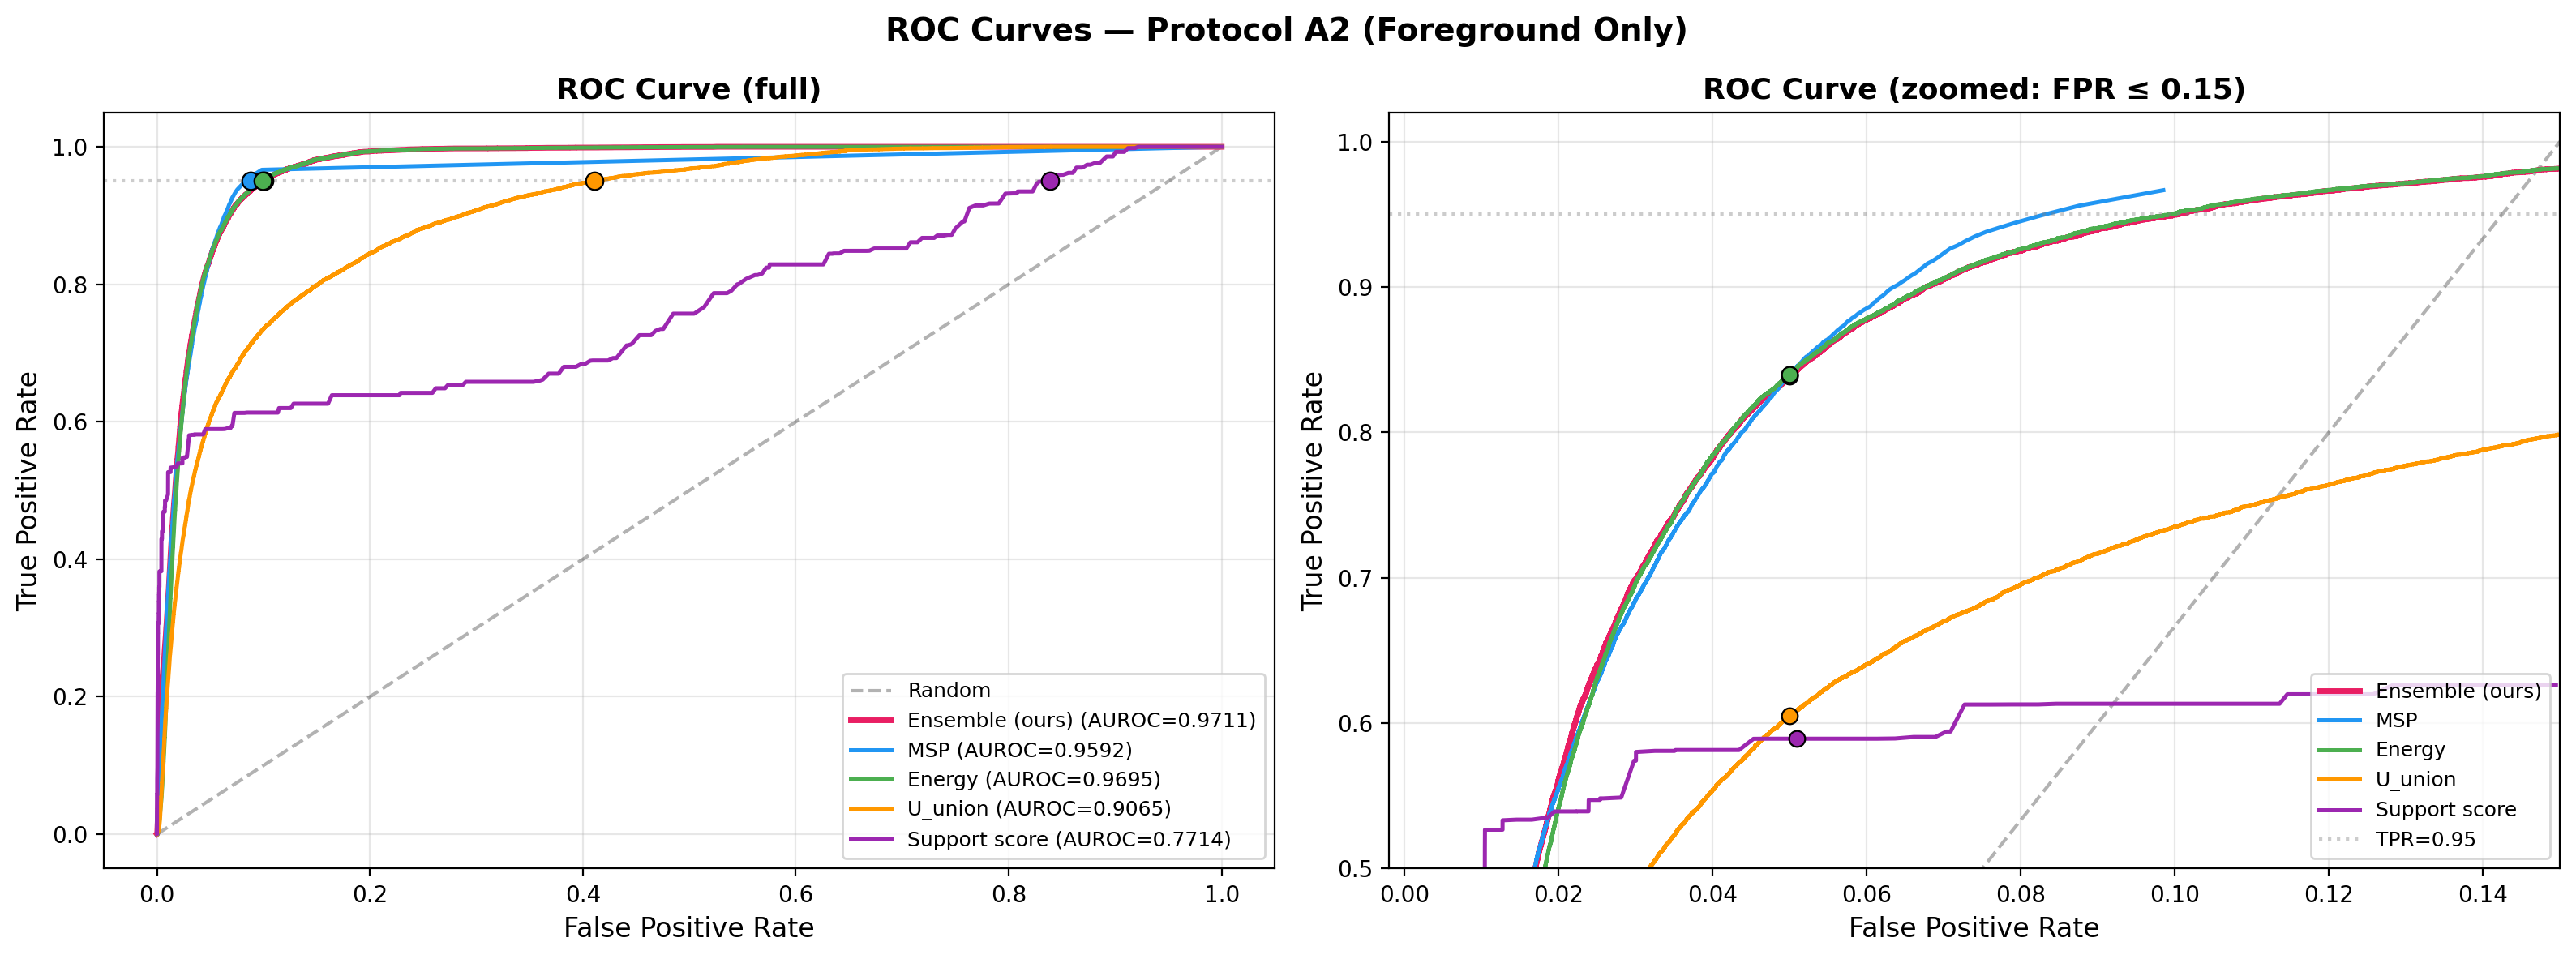
\includegraphics[width=\textwidth]{t3_roc_curve_a2.pdf}%
  }{%
    \IfFileExists{t3_roc_curve_a2.png}{%
      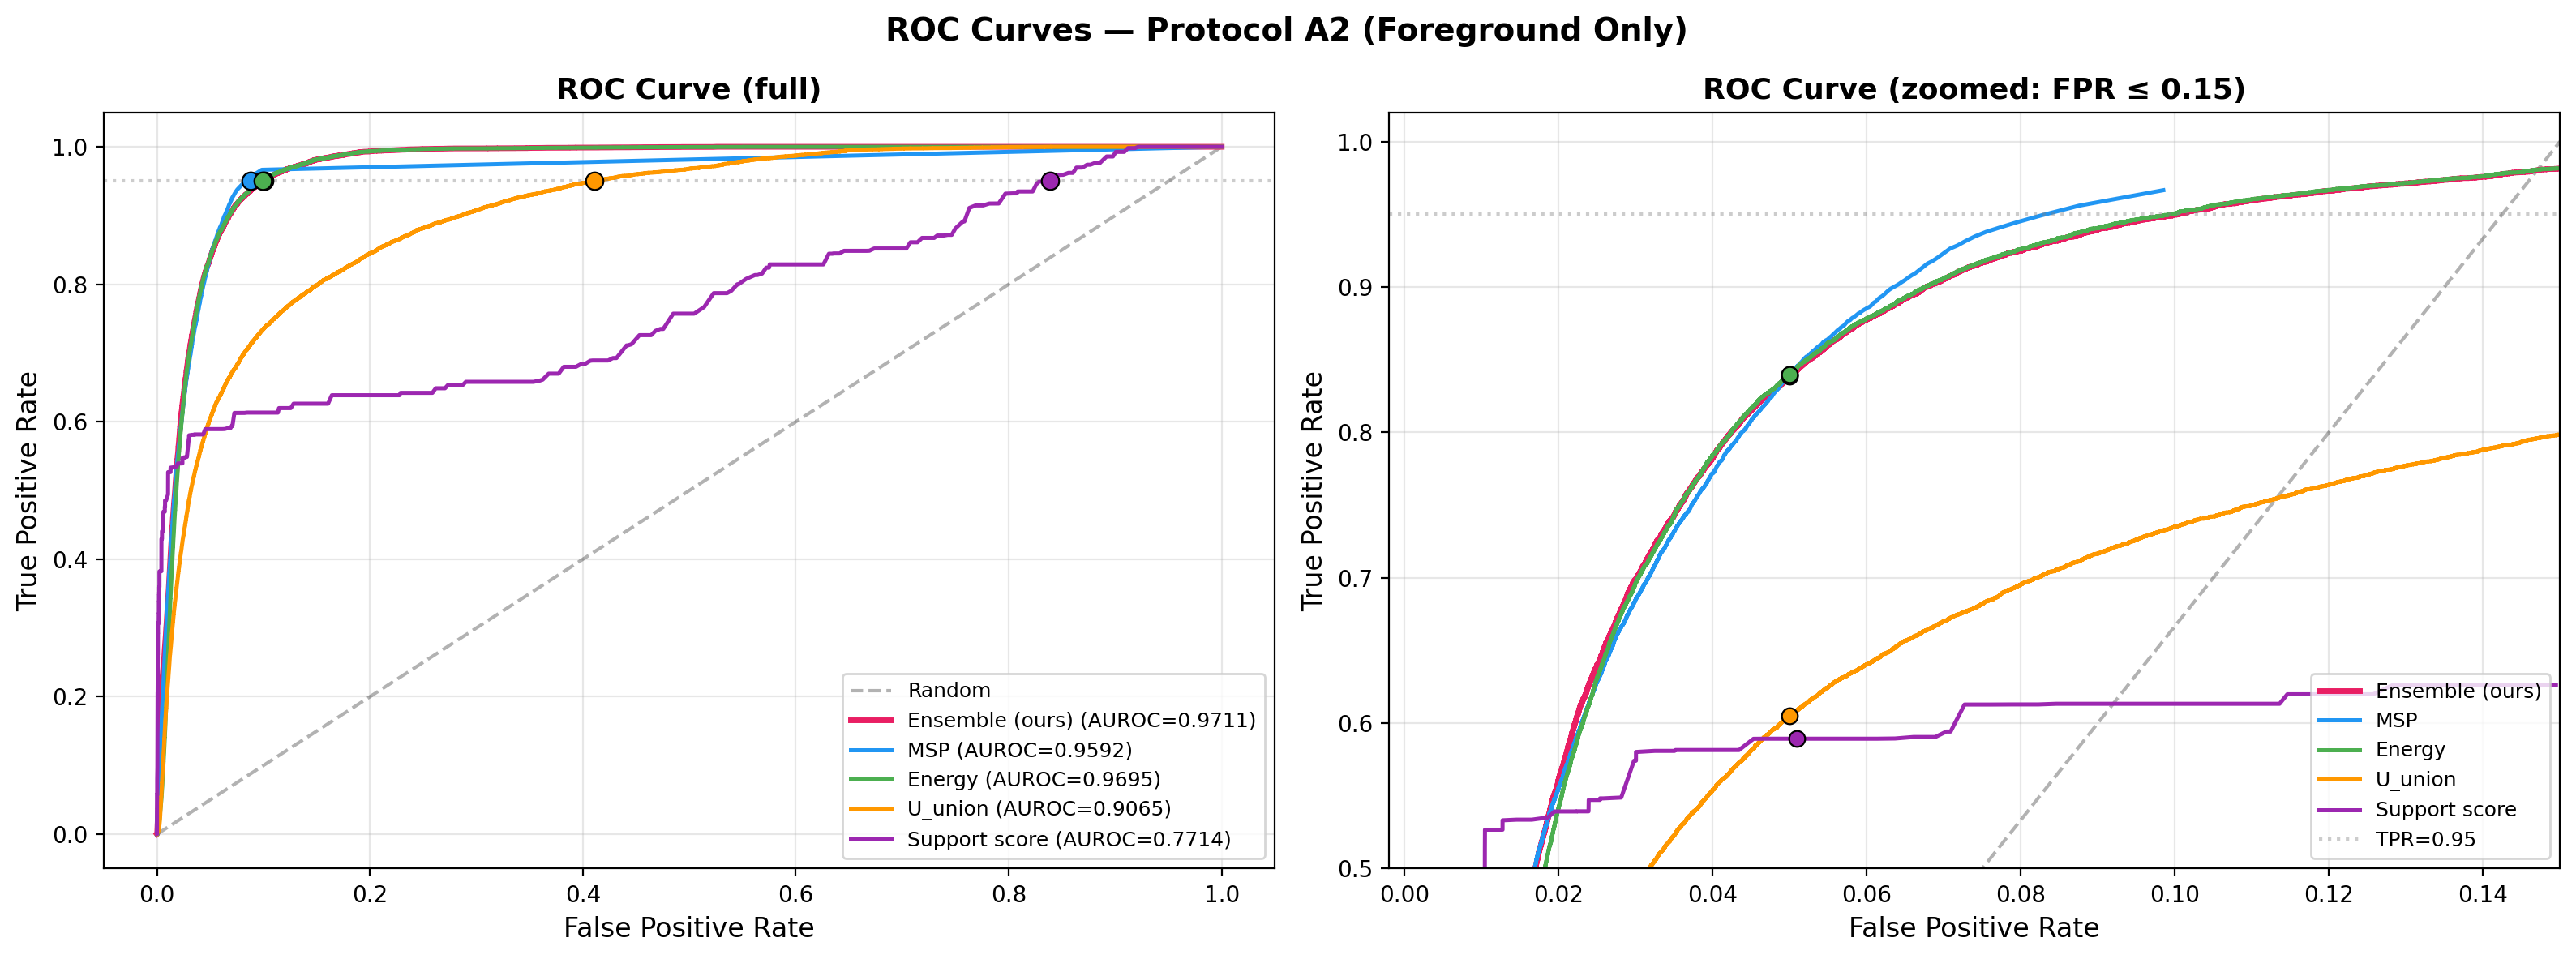
\includegraphics[width=\textwidth]{t3_roc_curve_a2.png}%
    }{%
      \fbox{\parbox{\textwidth}{\centering\vspace{4cm}ROC placeholder\vspace{4cm}}}%
    }%
  }
  \caption{ROC curves of different unknown detection signals under the Synapse A2 protocol (foreground pixels). Classification uncertainty signals (MSP, Energy, Ensemble) substantially outperform the geometric support score (Support) in global ranking.}\label{fig:a2_roc}
\end{figure*}

\begin{figure*}[!t]
  \centering
  \IfFileExists{t3_pr_curve_a2.pdf}{%
    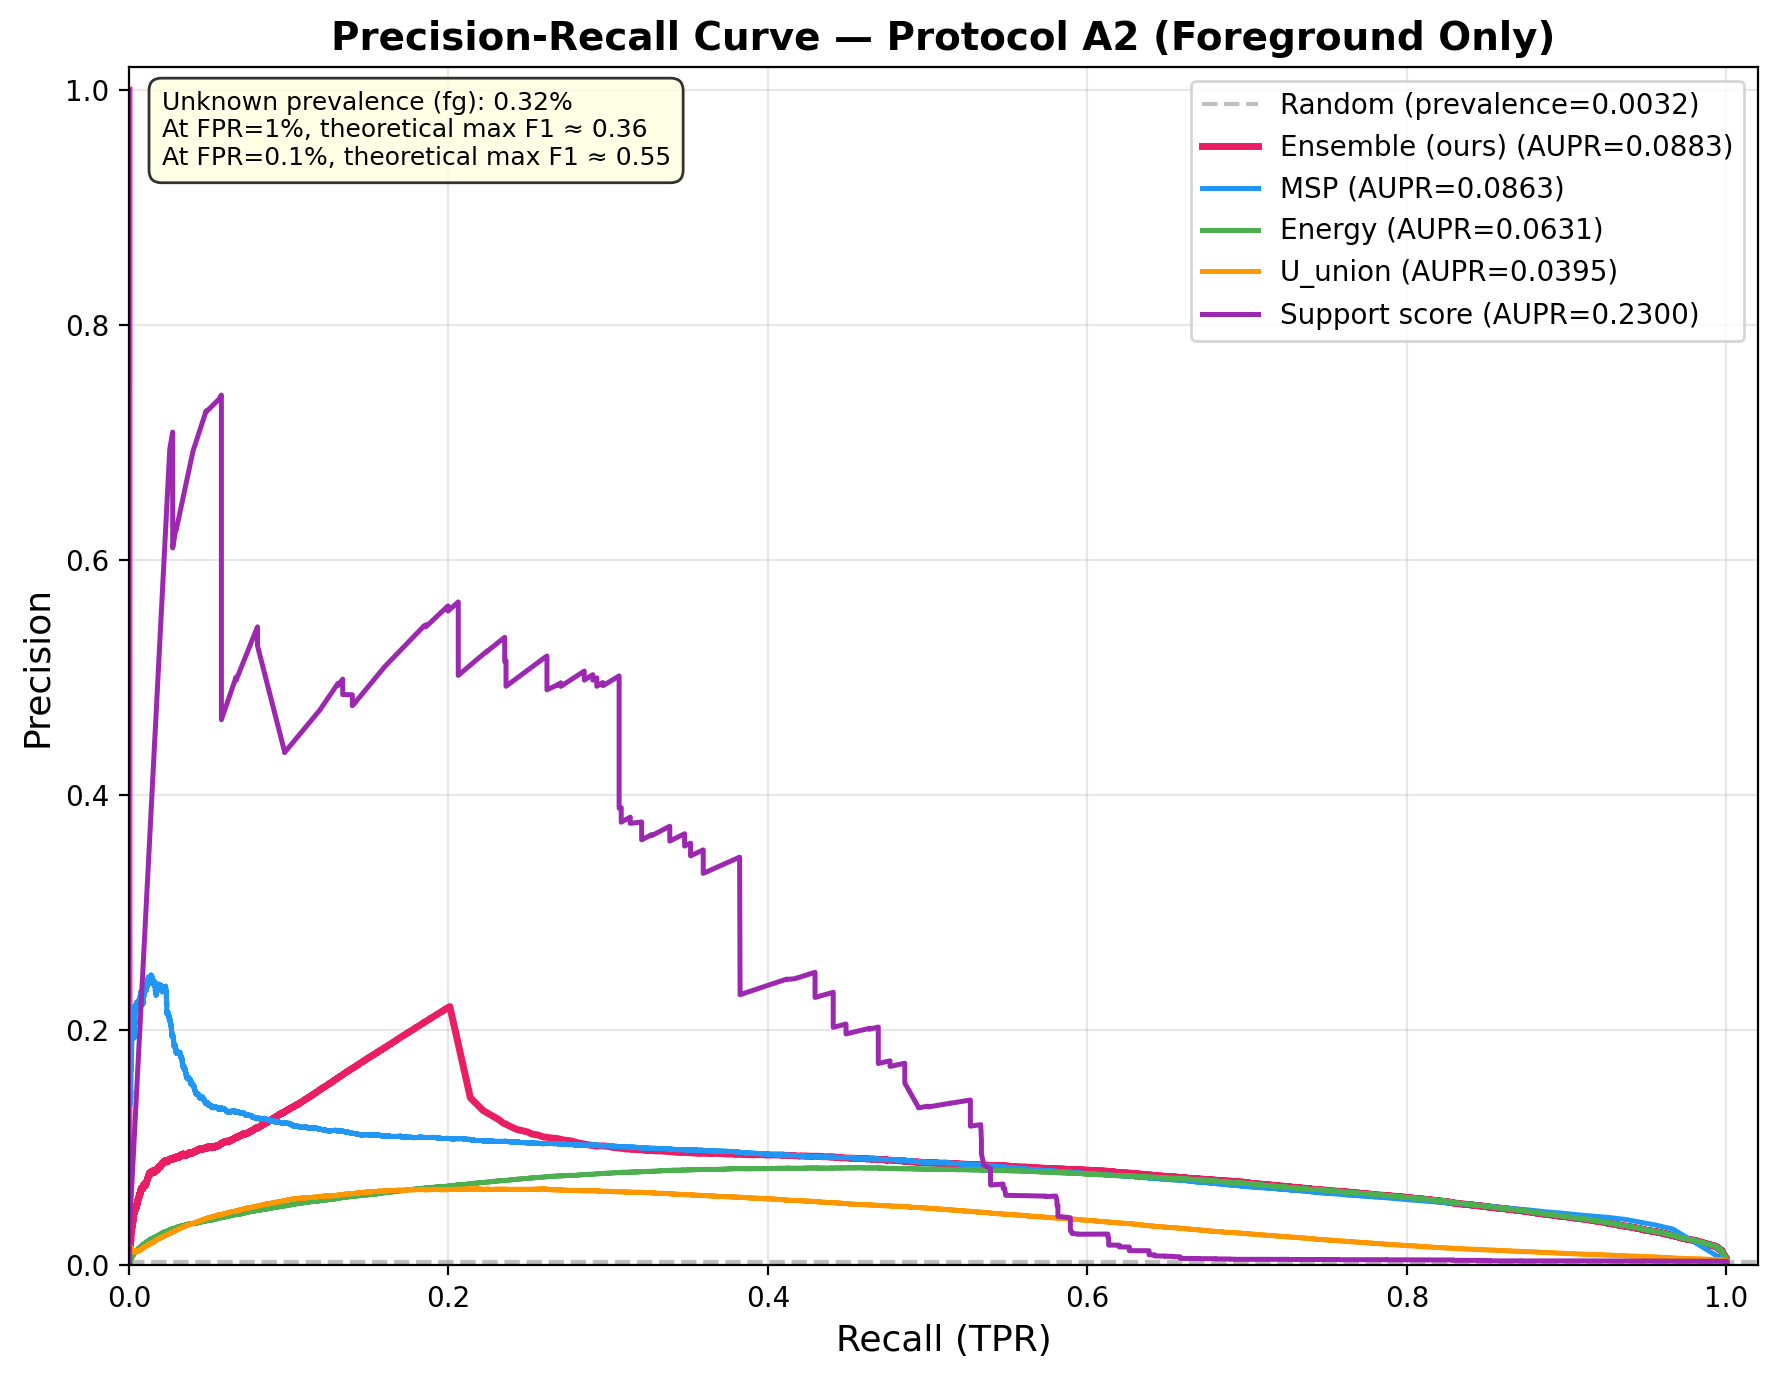
\includegraphics[width=\textwidth]{t3_pr_curve_a2.pdf}%
  }{%
    \IfFileExists{t3_pr_curve_a2.png}{%
      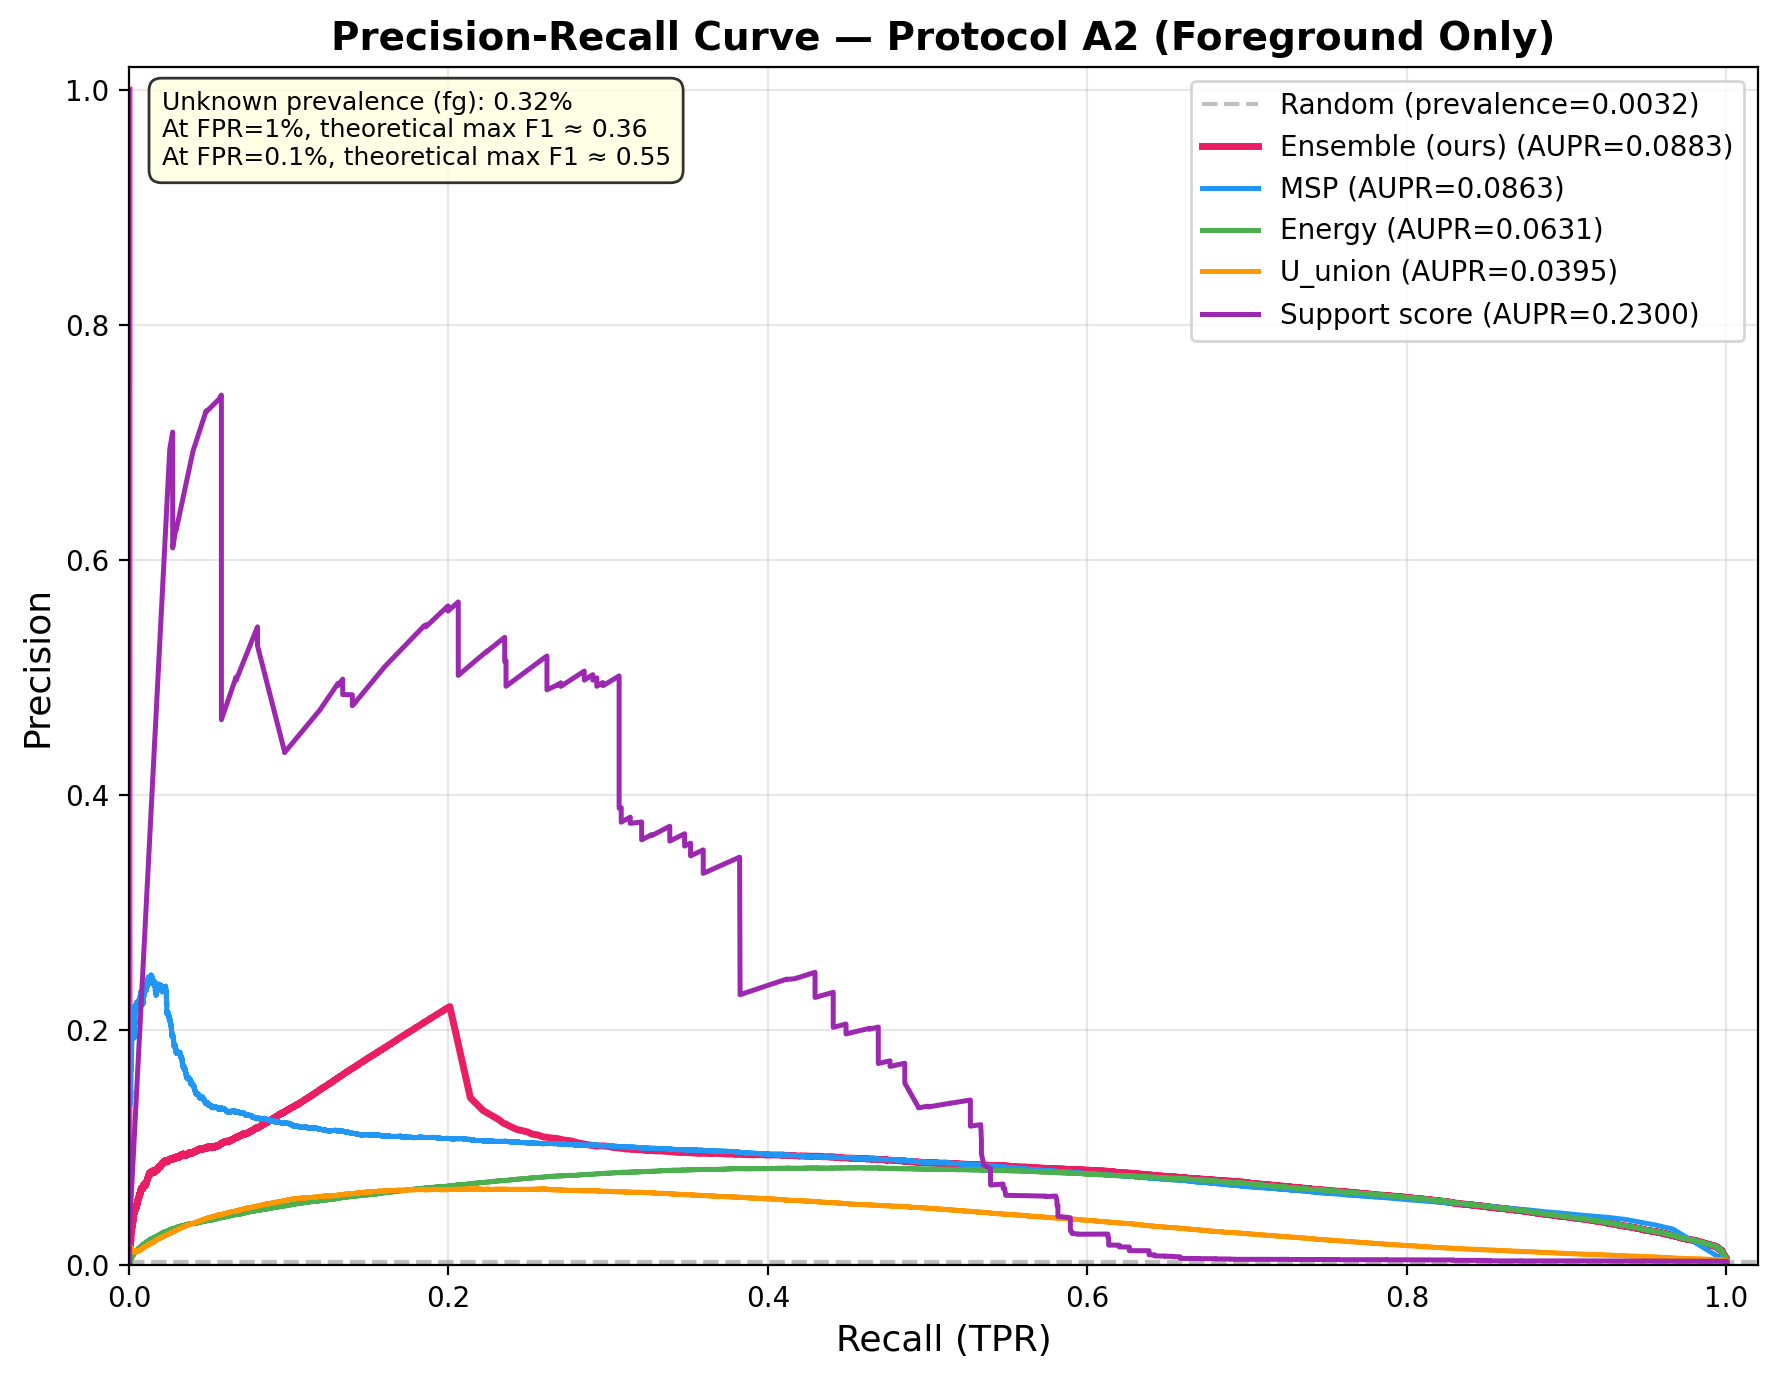
\includegraphics[width=\textwidth]{t3_pr_curve_a2.png}%
    }{%
      \fbox{\parbox{\textwidth}{\centering\vspace{4cm}PR placeholder\vspace{4cm}}}%
    }%
  }
  \caption{Precision--Recall curves of different unknown detection signals under the Synapse A2 protocol (foreground pixels). The Support score retains a local advantage in the high-precision regime, but its overall AUPR is constrained by limited global ranking capability.}\label{fig:a2_pr}
\end{figure*}


% ---------- 5.5 Ablation Studies ----------
\subsection{Ablation Studies}\label{sec:exp:ablation}

\subsubsection{Structural Ablation}\label{sec:exp:ablation:struct}

Table~\ref{tab:ablation} reports ablation results under the Synapse A1 protocol,
where model components or loss terms are modified one at a time (single seed, seed=42).

\begin{table}[t]
\centering
\footnotesize
\setlength{\tabcolsep}{4pt}
\caption{Structural ablation on Synapse A1. Baseline is the default configuration
($M=2, R=2$, full loss, no-object mechanism enabled). Each row modifies one variable.}\label{tab:ablation}
\resizebox{\columnwidth}{!}{%
\begin{tabular}{lcc}
\toprule
Setting & Known mIoU & Unknown F1 \\
\midrule
Baseline ($M=2, R=2$) & $0.811$ & $0.721$ \\
\midrule
$M=1$ & $0.814$ & $0.697$ \\
$M=4$ & $0.810$ & $0.711$ \\
\midrule
$R=1$ & $0.800$ & $0.670$ \\
$R=4$ & $0.812$ & $0.713$ \\
\midrule
w/o $\mathcal{L}_{\text{ball}}$ & $0.797$ & $0.662$ \\
w/o $\mathcal{L}_{\text{boundary}}$ & $0.813$ & $0.724$ \\
w/o no-object & $0.814$ & $0.709$ \\
\bottomrule
\end{tabular}
}
\end{table}

Key findings are as follows.

\paragraph{Number of Unknown Slots ($M$)}
$M=2$ is the optimal configuration (F1=0.721); $M=1$ degrades substantially to 0.697
($-$2.4pp), while $M=4$ yields no further improvement (0.711).
This indicates that two slots are sufficient to cover the spatial diversity of unknown
regions on a single slice, and additional slots introduce redundancy.

\paragraph{Number of Prototype Spheres ($R$)}
$R=1$ (single prototype) causes simultaneous declines in both known mIoU and unknown F1
(mIoU $-$1.1pp, F1 $-$5.1pp); $R=4$ shows no appreciable improvement over $R=2$.
This validates the effectiveness of $R=2$ in covering the bimodal distribution of organ
slice positions.

\paragraph{Loss Function}
Removing $\mathcal{L}_{\text{ball}}$ causes the largest drop in unknown F1 ($-$5.9pp)
as well as a 1.4pp decrease in known mIoU, indicating that geometric constraints
benefit not only unknown determination but also have an indirect positive effect on
known-class representation quality.
Removing $\mathcal{L}_{\text{boundary}}$ has negligible impact on F1 (+0.3pp) but
shifts precision from 0.775 to 0.796 and recall from 0.674 to 0.664, suggesting
that this term primarily modulates the precision--recall trade-off rather than
significantly altering overall F1 in the current setting.
Removing the no-object mechanism leads to a modest F1 decline of 1.2pp.

\subsubsection{$M=0$ Core Ablation: Necessity of Native Unknown Queries}\label{sec:exp:ablation:m0}

Table~\ref{tab:m0} reports results after completely removing unknown queries ($M=0$),
which constitutes the most critical ablation experiment of this paper.

\begin{table}[t]
\centering
\footnotesize
\setlength{\tabcolsep}{3pt}
\caption{$M=0$ ablation: can post-hoc signals substitute for structured abstention
after removing native unknown queries?
Synapse A1 protocol. `\texttt{---}' indicates the metric is not applicable or not
reported for that setting.}\label{tab:m0}
\resizebox{\columnwidth}{!}{%
\begin{tabular}{lccc}
\toprule
Setting & Known mIoU & Unknown F1 & AUROC$_{\text{fg}}$ \\
\midrule
$M=2$ + $U_{\text{union}}$ & $0.809$ & $\mathbf{0.728}$ & --- \\
$M=2$ + Support & $0.811$ & $0.721$ & --- \\
\midrule
$M=0$ + MSP & $0.782$ & $0.070$ & $0.965$ \\
$M=0$ + Prototype-sphere & $0.791$ & $0.008$ & $0.562$ \\
\bottomrule
\end{tabular}
}
\end{table}

The results are decisive.
\textbf{Upon removing unknown queries, unknown F1 collapses catastrophically from
0.721--0.728 to 0.008--0.070} (a reduction exceeding 90\%), while known mIoU
decreases by only approximately 2\%.
Notably, $M=0$ + MSP still achieves a pixel-level AUROC of 0.965, demonstrating
that post-hoc signals remain effective at pixel-level \textbf{ranking}---but they
cannot translate this ranking capability into spatially coherent unknown masks.

\textbf{This ablation directly demonstrates that, within our framework, post-hoc
signals alone are insufficient to substitute for an explicit unknown output space
after unknown queries are removed.}
Combined with the independent baseline comparison in Section~\ref{sec:exp:indep},
it can be seen that the truly critical factor in A1 is whether an explicit unknown
output space is reserved, not merely whether a query-based or per-pixel implementation
is adopted.

\paragraph{Split Robustness Validation}
To verify whether the above conclusions depend on a particular seen/unseen class
partition, we construct an alternative split (alt-split): one pathological class from
the original unseen side (liver tumor, label 12) is moved to the seen side, while
one anatomical class from the original seen side (pancreas, label 11) is moved to the
unseen side, deliberately crossing the semantic boundary of the original split.
Table~\ref{tab:alt_split} compares the $M=0$ ablation results under both splits.

\begin{table}[t]
\centering
\footnotesize
\setlength{\tabcolsep}{3pt}
\caption{Split robustness validation: the $M=0$ collapse remains after replacing the seen/unseen split.
Synapse A1 protocol.}\label{tab:alt_split}
\begin{tabular}{llcc}
\toprule
Split & Setting & Known mIoU & Unknown F1 \\
\midrule
Original & $M=2$ (Support) & $0.811$ & $0.721$ \\
Original & $M=0$ (MSP) & $0.782$ & $0.070$ \\
\midrule
Alt-split & $M=2$ (Support) & $0.819$ & $0.787$ \\
Alt-split & $M=0$ (MSP) & $0.831$ & $0.043$ \\
\bottomrule
\end{tabular}
\end{table}

Under the alt-split, unknown F1 collapses from 0.787 to 0.043 (a reduction of 94.6\%),
even greater than the 90.3\% under the original split, while known mIoU remains stable.
This demonstrates that the mechanism revealed by the $M=0$ ablation---that removing
unknown queries causes structured abstention capability to collapse---is
not contingent on any particular class partition scheme.

Figure~\ref{fig:m0_vis} shows a qualitative comparison between $M=2$ and $M=0$.
The $M=2$ model produces coherent segmentation masks in unknown regions, while the
post-hoc results of the $M=0$ model are fragmented and fail to form meaningful regions.

\begin{figure*}[!t]
  \centering
  \IfFileExists{t2_m2_vs_m0_grid.pdf}{%
    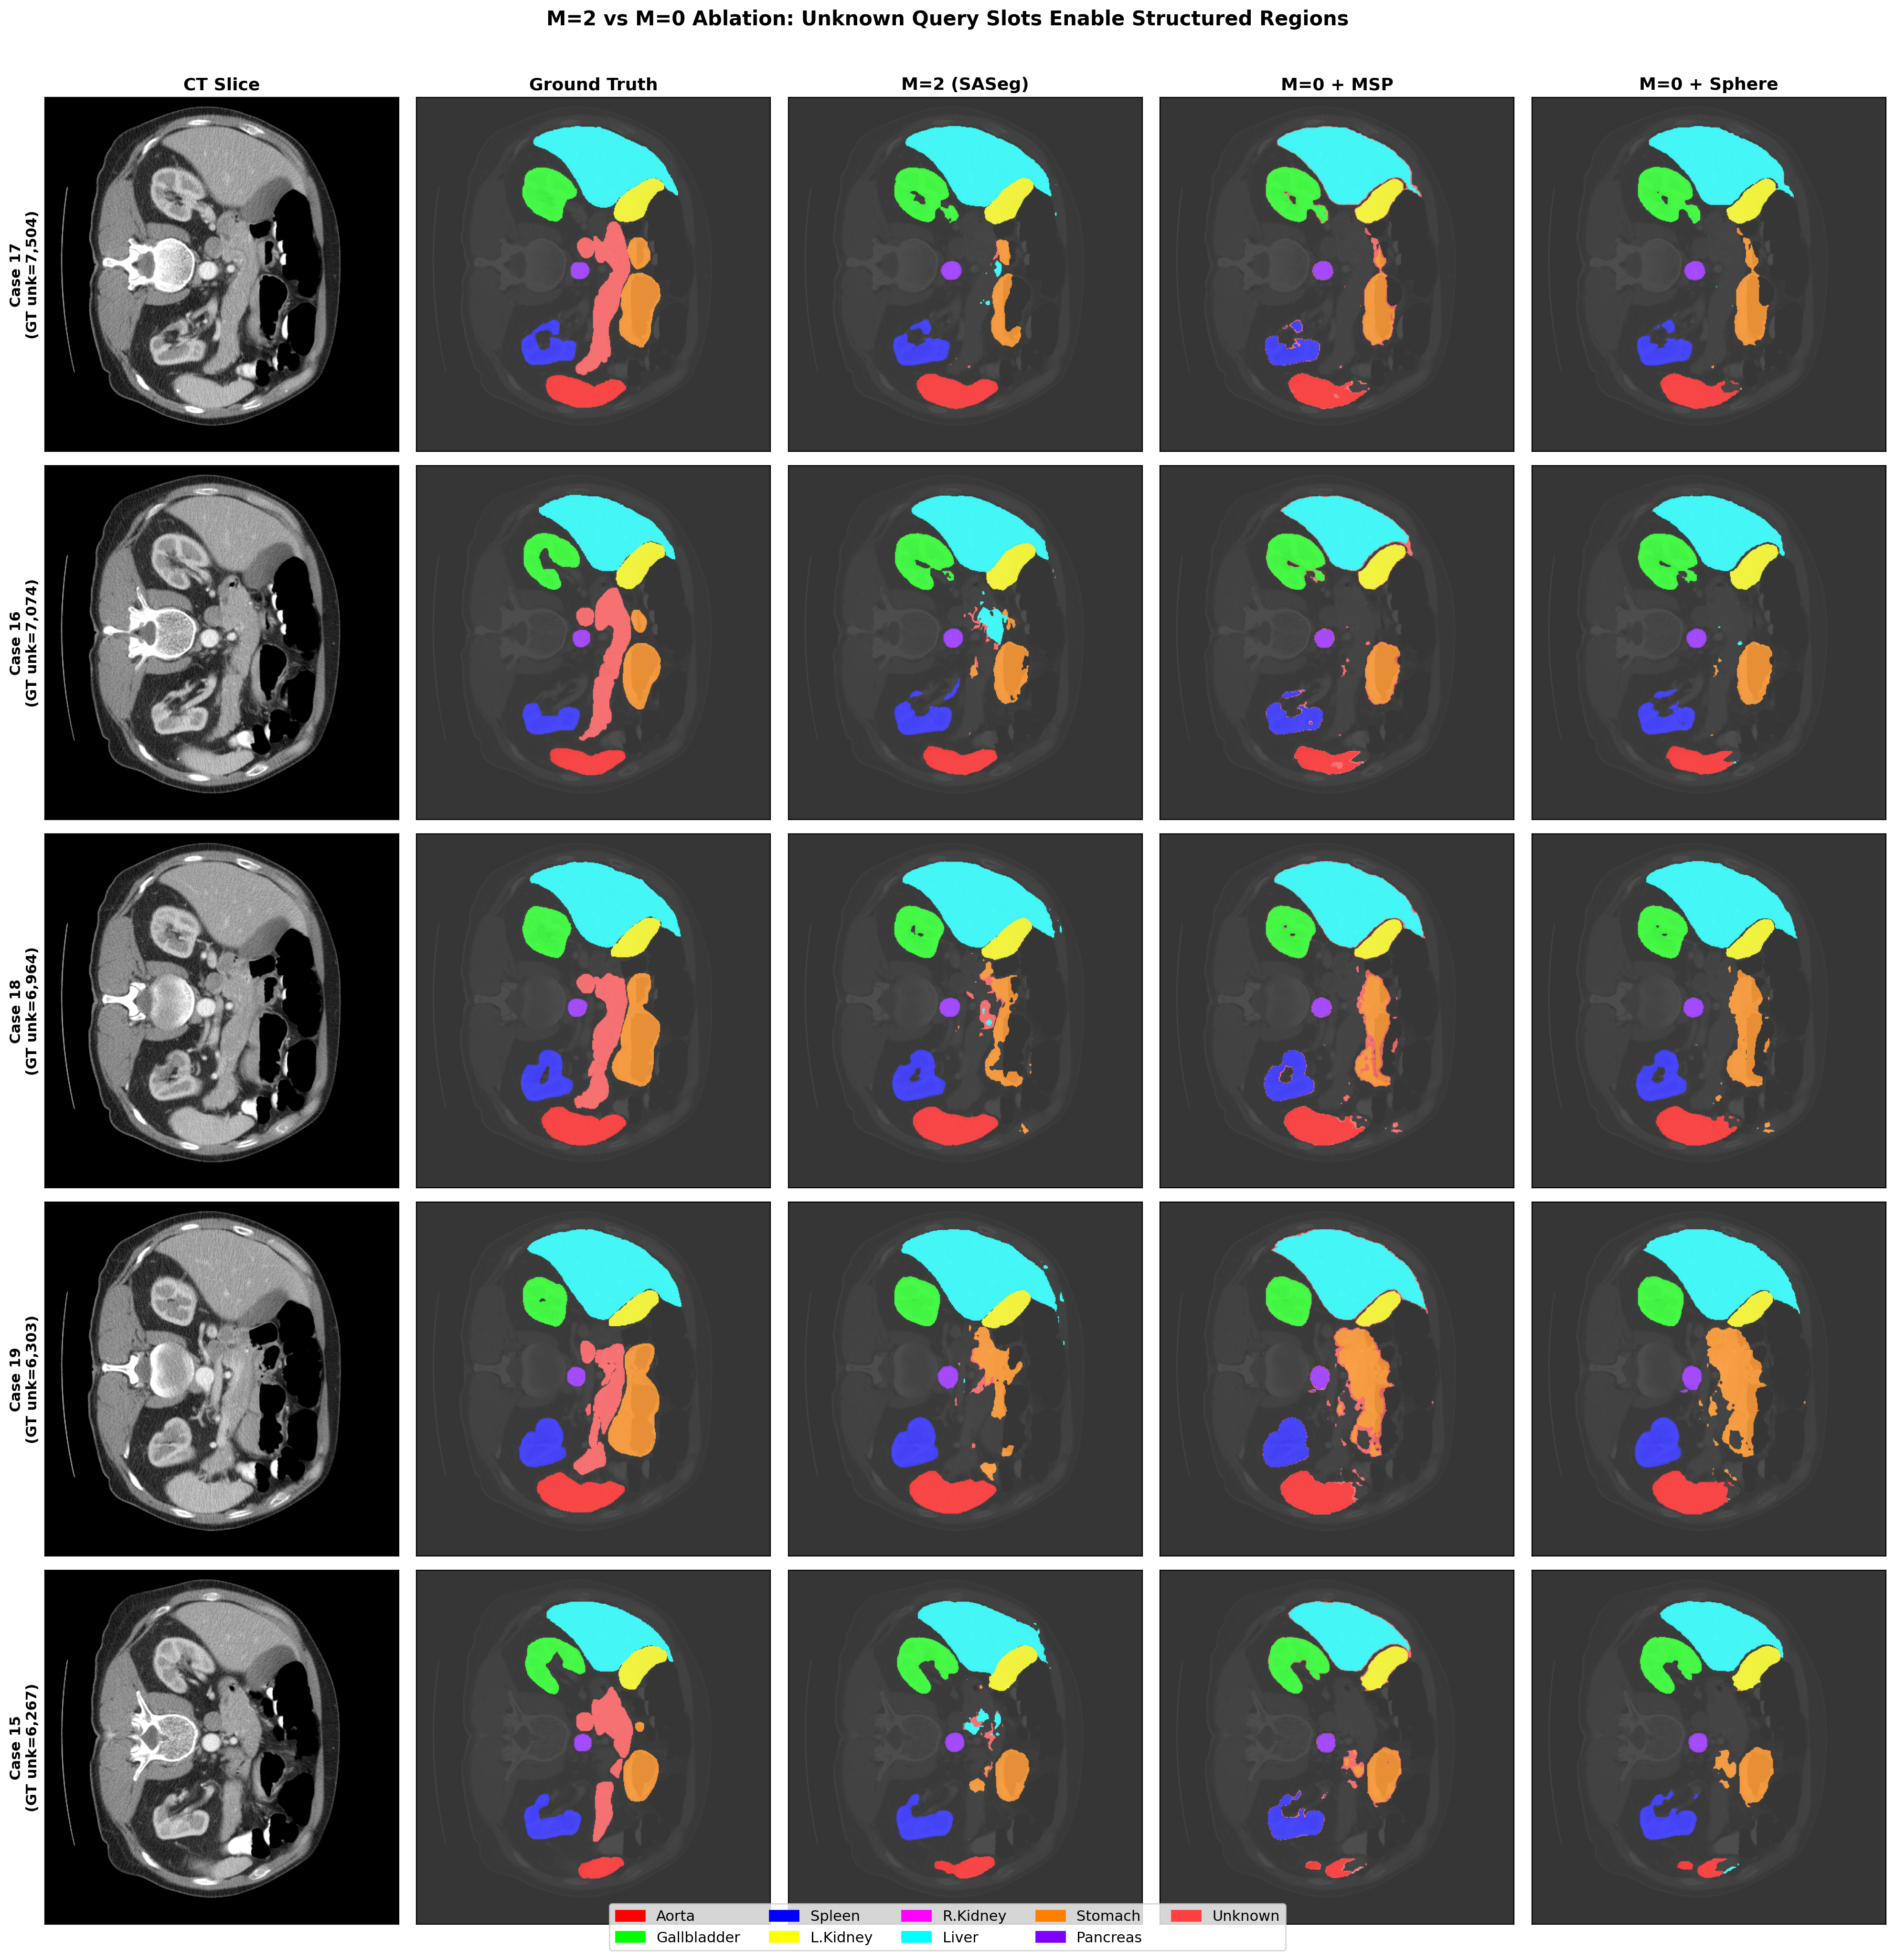
\includegraphics[width=\textwidth]{t2_m2_vs_m0_grid.pdf}%
  }{%
    \IfFileExists{t2_m2_vs_m0_grid.png}{%
      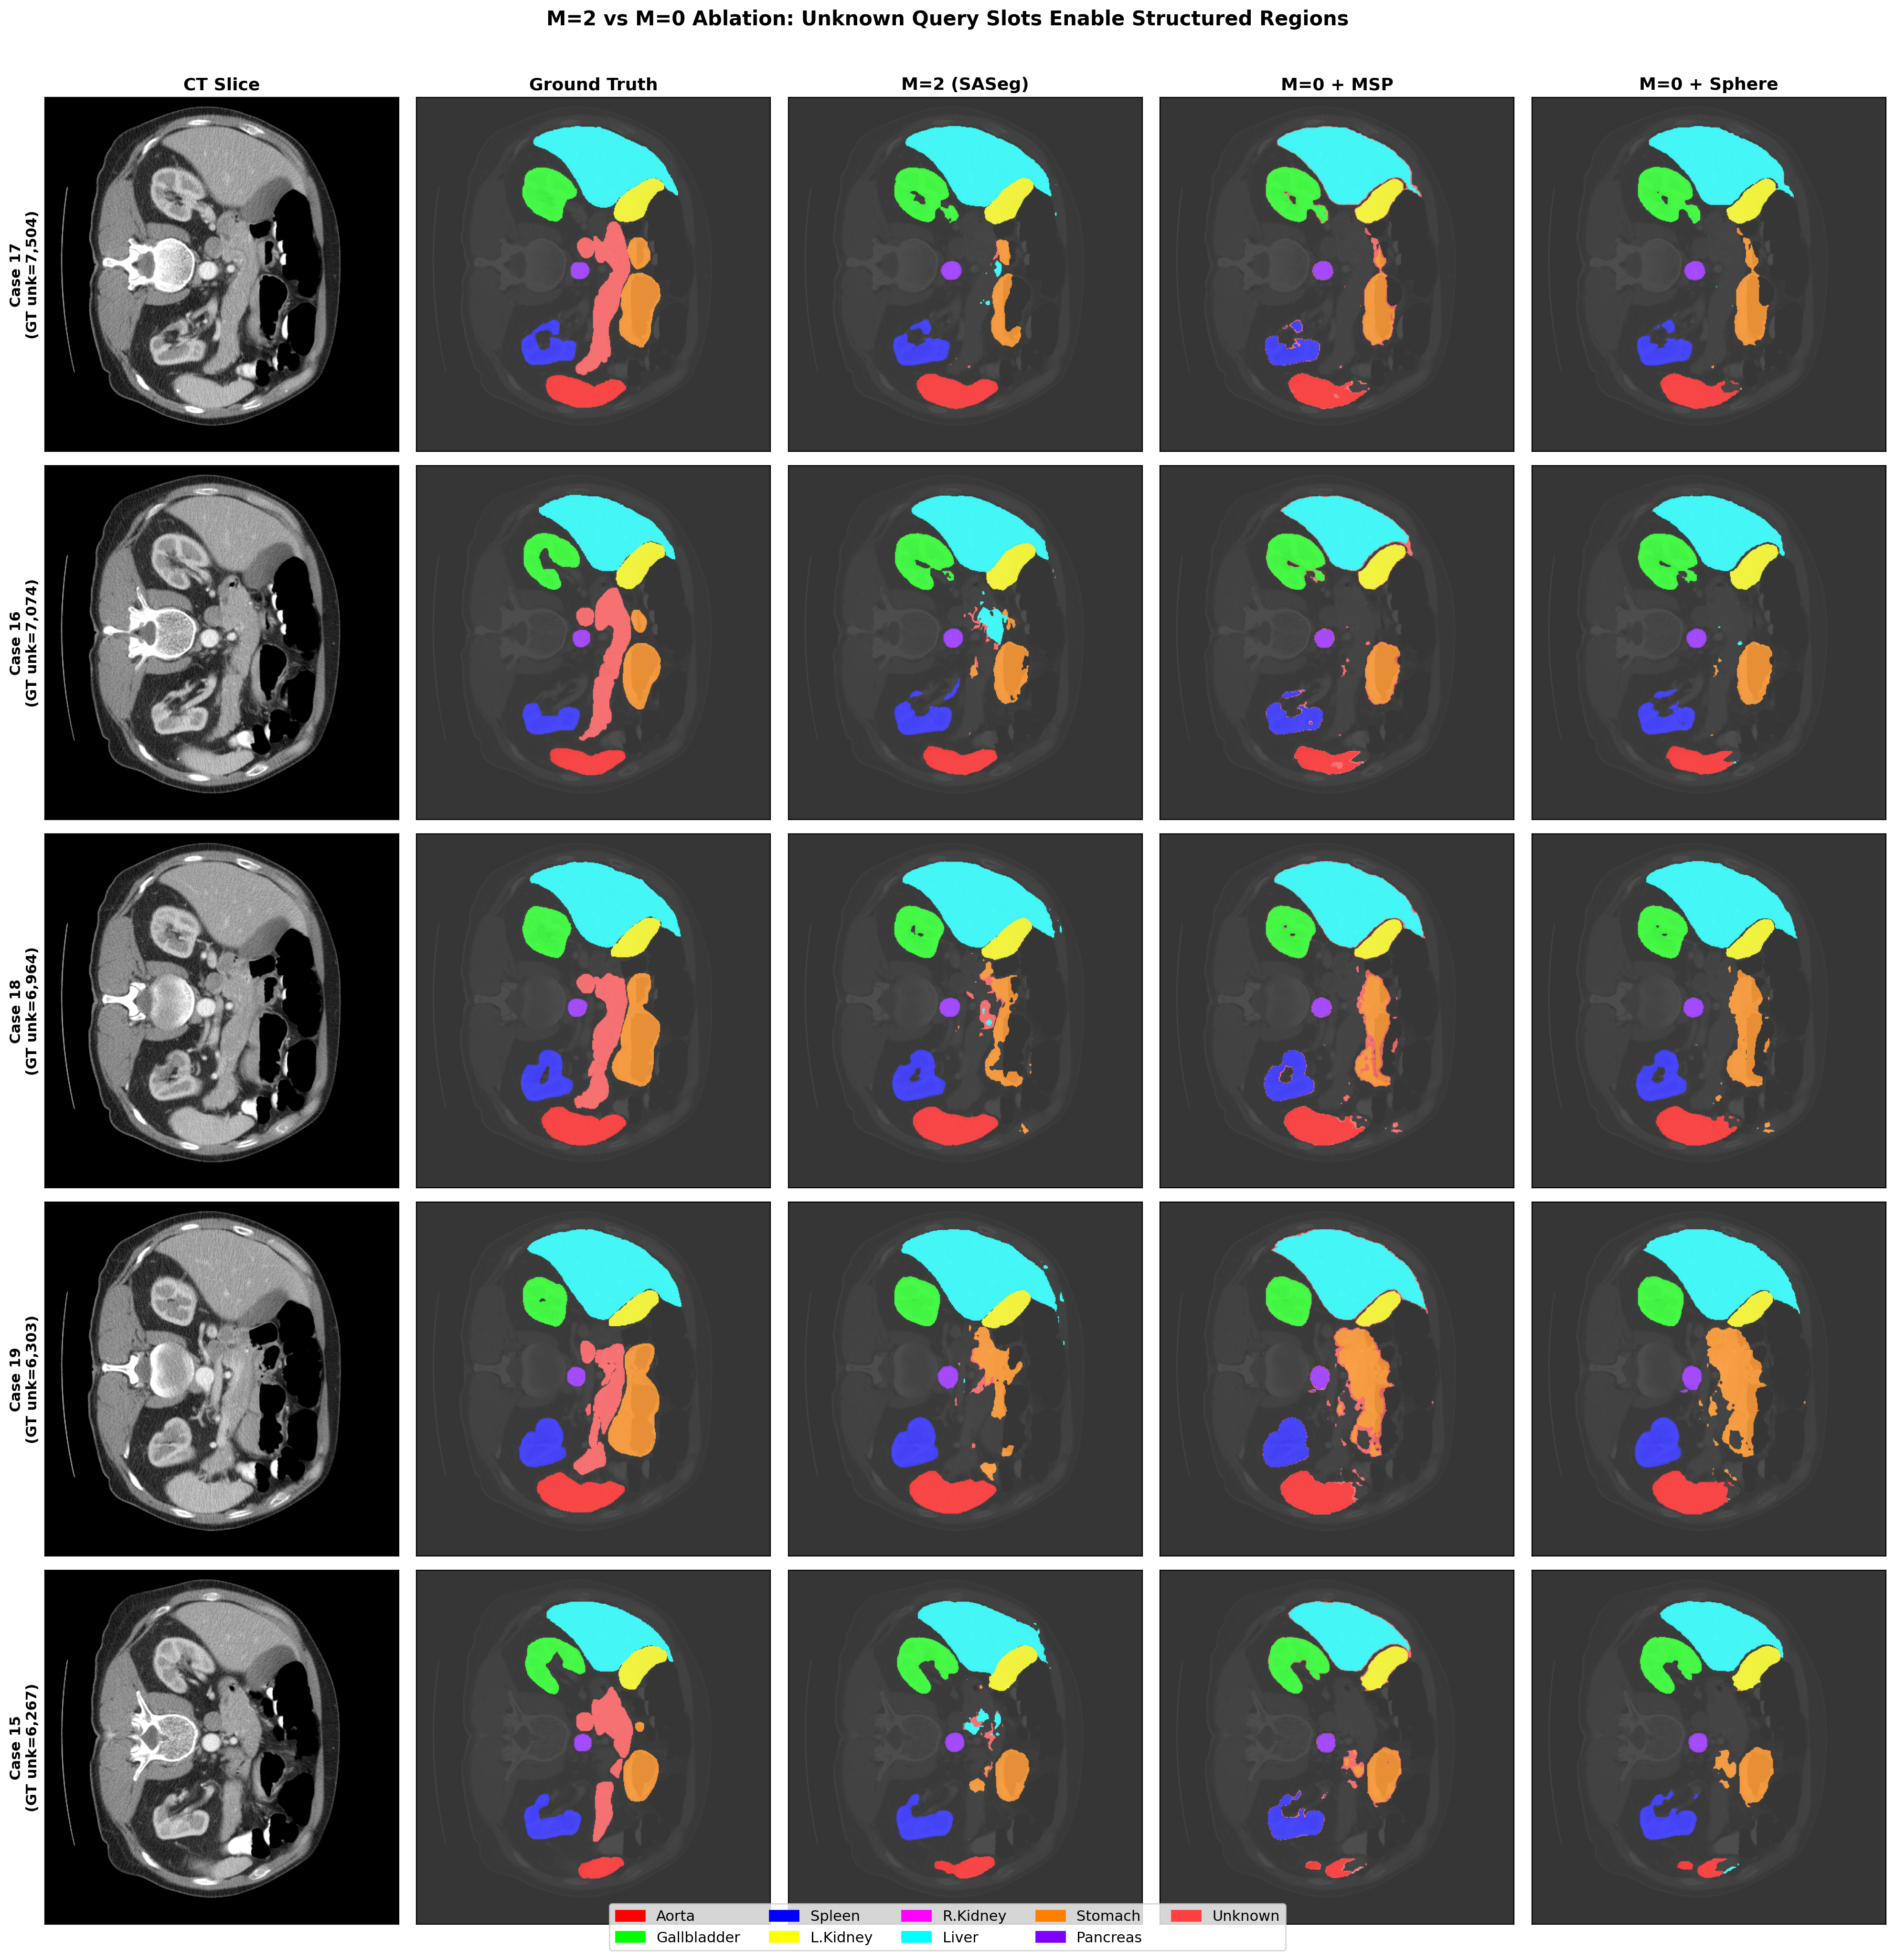
\includegraphics[width=\textwidth]{t2_m2_vs_m0_grid.png}%
    }{%
      \fbox{\parbox{\textwidth}{\centering\vspace{4cm}$M=2$ vs $M=0$ qualitative comparison placeholder\vspace{4cm}}}%
    }%
  }
  \caption{Qualitative comparison of $M=2$ (top) and $M=0$ (bottom) on Synapse A1.
  The $M=2$ model produces spatially coherent unknown masks (in red) via native unknown
  queries, while the post-hoc unknown determination of the $M=0$ model exhibits a
  fragmented distribution that fails to form structured abstention outputs.}\label{fig:m0_vis}
\end{figure*}


% ---------- 5.6 Cross-Dataset Validation ----------
\subsection{Cross-Dataset Validation: AMOS22}\label{sec:exp:cross}

To validate the cross-dataset consistency of the core conclusions, we reproduce three
key experiments on the AMOS22 CT subset: A1, A2, and the $M=0$ ablation.
The CT-only setting is used, with annotated CT training and validation sets comprising
200 and 100 cases, respectively; AMOS22 results are from independent training followed
by validation set evaluation, not merely used as a validation split.
AMOS22 contains 15-class organ annotations, split as $K=8$ (known) / 4 (seen unknown) /
3 (unseen unknown).

Table~\ref{tab:cross} summarizes the cross-dataset comparison results.

\begin{table*}[!t]
\centering
\caption{Cross-dataset comparison between Synapse and AMOS22.
All three core conclusions are consistent across both independent datasets.
`\texttt{---}' indicates the metric is not applicable or not reported for that setting.}\label{tab:cross}
\footnotesize
\resizebox{\textwidth}{!}{%
\begin{tabular}{ll ccc cc c}
\toprule
Experiment & Dataset & mIoU$_{\text{K}}$ & F1$_{\text{U}}$ & IoU$_{\text{U}}$ & Prec$_{\text{U}}$ & Rec$_{\text{U}}$ & AUROC$_{\text{fg}}$ \\
\midrule
\multirow{2}{*}{A1} & Synapse & $0.811$ & $0.721$ & $0.564$ & $0.775$ & $0.674$ & --- \\
                     & AMOS22  & $0.838$ & $0.839$ & $0.723$ & $0.848$ & $0.831$ & --- \\
\midrule
\multirow{2}{*}{A2 (Ens.)} & Synapse & $0.797$ & $0.006$ & $0.003$ & --- & --- & $0.971$ \\
                            & AMOS22  & $0.827$ & $0.010$ & $0.005$ & $0.006$ & $0.025$ & $0.990$ \\
\midrule
\multirow{2}{*}{$M\!=\!0$+MSP} & Synapse & $0.782$ & $0.070$ & --- & --- & --- & $0.965$ \\
                                 & AMOS22  & $0.814$ & $0.045$ & $0.023$ & $0.059$ & $0.037$ & $0.983$ \\
\multirow{2}{*}{$M\!=\!0$+Sph.} & Synapse & $0.791$ & $0.008$ & --- & --- & --- & $0.562$ \\
                                  & AMOS22  & $0.816$ & $0.017$ & $0.009$ & $0.077$ & $0.010$ & $0.780$ \\
\bottomrule
\end{tabular}%
}
\end{table*}

All three core conclusions hold across datasets:

\paragraph{A1 Structured Abstention is Effective}
AMOS22 A1 achieves unknown F1 of 0.839, even higher than Synapse (0.721),
while known mIoU is maintained at 0.838.
This demonstrates that the framework's structured abstention capability remains
effective on a larger-scale dataset, and indeed exhibits stronger performance.

\paragraph{Detection $\neq$ Structuring in A2}
AMOS22 A2 Ensemble AUROC$_{\text{fg}}$ reaches 0.990 (vs.\ 0.971 on Synapse),
yet unknown F1 is only 0.010, entirely consistent with the Synapse trend.
This confirms that ``high detection ranking $\neq$ usable structured abstention output''
is not an incidental Synapse artifact, but an inherent characteristic of the
unseen-unknown setting.

\paragraph{$M=0$ Ablation Cross-Dataset Confirmed}
On AMOS22, removing unknown queries causes F1 to collapse from 0.839 to 0.045 (MSP)
/ 0.017 (Sphere), reductions of 94.6\% and 98.0\% respectively, fully consistent in
direction with Synapse.
The necessity of native unknown queries for structured abstention is validated on two
independent datasets.


% ---------- 5.7 Cross-Domain Generalization ----------
\subsection{Cross-Domain Generalization Beyond Medical CT}\label{sec:exp:crossdomain}

The experiments above demonstrate structured abstention on medical CT.
A natural question is whether the two core phenomena---the necessity of native unknown
slots and the detection--structuring gap---depend on CT-specific image statistics or
are general properties of dense segmentation.
To answer this, we reproduce the minimal set of experiments (A1 + $M{=}0$ ablation,
and A2) on two natural-image benchmarks with visual characteristics markedly different
from abdominal CT.
We do \emph{not} reproduce the full ablation suite or conduct baseline comparisons
on these datasets; the goal is strictly to confirm directional consistency of the
two core phenomena.

\subsubsection{Datasets and Protocol Splits}\label{sec:exp:crossdomain:data}

\paragraph{PASCAL VOC 2012}
We use the standard PASCAL VOC 2012 segmentation split (1,464 training / 1,449 validation
images, 20 foreground semantic classes)~\cite{everingham2010pascal}.
The known/unknown split follows the same semantic-grouping principle as the medical
datasets:
\begin{itemize}[nosep]
  \item Known $\cK$ (15 classes): aeroplane, bicycle, bird, boat, bottle, bus, car, cat,
        chair, cow, diningtable, dog, horse, person, pottedplant.
  \item Seen unknowns $\cU_{\text{seen}}$ (3 classes): sheep, sofa, train---regularly
        occurring categories withheld from the known label set, providing structured
        abstention supervision during A1 training.
  \item Unseen unknowns $\cU_{\text{unseen}}$ (2 classes): motorbike, tvmonitor---selected
        for their visual proximity to known classes (motorbike $\leftrightarrow$ bicycle;
        tvmonitor $\leftrightarrow$ chair/indoor objects), making A2 a non-trivial
        detection task.
\end{itemize}

\paragraph{Cityscapes}
We use the standard Cityscapes fine-annotation split (2,975 training / 500 validation
images, 19 semantic classes) in the single-scale evaluation setting~\cite{cordts2016cityscapes}.
The split is:
\begin{itemize}[nosep]
  \item Known $\cK$ (14 classes): road, sidewalk, building, wall, fence, pole,
        traffic light, traffic sign, vegetation, terrain, sky, car, person, rider.
  \item Seen unknowns $\cU_{\text{seen}}$ (3 classes): truck, bus, train---large
        vehicles that are visible during training but excluded from the known output space.
  \item Unseen unknowns $\cU_{\text{unseen}}$ (2 classes): motorcycle, bicycle---
        fine-grained two-wheeled participants that share visual similarity with
        person/rider/car and are entirely absent from the A2 training set.
\end{itemize}
Dataset-internal void/ignore labels are excluded and do not contribute to any
unknown category.
All other training configurations (encoder, loss weights, epochs, augmentations)
follow the same defaults as the medical experiments (Section~\ref{sec:exp:setup:impl}).

\subsubsection{Native Unknown Slot Necessity Across Domains}\label{sec:exp:crossdomain:m0}

Table~\ref{tab:crossdomain_m0} reports A1 and $M{=}0$ ablation results on both
natural-image datasets.

\begin{table}[!t]
\centering
\caption{A1 structured abstention and $M{=}0$ ablation on PASCAL VOC and Cityscapes.
Native unknown slots are necessary for structured abstention in both natural-image
settings: removing them ($M{=}0$) collapses unknown F1 by over 96\%, even when the
replacement scoring signal (MSP) retains strong pixel-level ranking (AUROC $>$ 0.93).}
\label{tab:crossdomain_m0}
\footnotesize
\begin{tabular}{ll ccc}
\toprule
Dataset & Setting & mIoU$_{\text{K}}$ & F1$_{\text{U}}$ & AUROC$_{\text{fg}}$ \\
\midrule
\multirow{3}{*}{VOC}
  & A1 ($M{=}2$)       & $0.780$ & $0.813$ & --- \\
  & $M{=}0$ + MSP      & $0.627$ & $0.027$ & $0.934$ \\
  & $M{=}0$ + Sphere   & $0.649$ & $0.000$ & $0.698$ \\
\midrule
\multirow{3}{*}{Cityscapes}
  & A1 ($M{=}2$)       & $0.642$ & $0.737$ & --- \\
  & $M{=}0$ + MSP      & $0.590$ & $0.024$ & $0.956$ \\
  & $M{=}0$ + Sphere   & $0.592$ & $0.000$ & $0.473$ \\
\bottomrule
\end{tabular}
\end{table}

On both datasets, the $M{=}0$ ablation produces the same collapse pattern observed
on Synapse and AMOS22.
On VOC, unknown F1 drops from 0.813 to 0.027 under MSP and to 0.000 under
Prototype-sphere, reductions of 96.7\% and 100\% respectively.
On Cityscapes, the drop is from 0.737 to 0.024 (MSP, $-$96.8\%) and 0.000 (Sphere).
Crucially, MSP retains strong pixel-level AUROC (0.934 on VOC, 0.956 on Cityscapes),
demonstrating that the collapse is not caused by a failure of the scoring signal to
rank unknown pixels---the signal can still rank them well---but by the absence of a
native structured output slot to aggregate those pixels into coherent regions.
Known mIoU decreases moderately under $M{=}0$ ($-0.153$ on VOC, $-0.052$ on
Cityscapes), similar in pattern to the medical experiments.
These results confirm that the necessity of native unknown slots for structured
abstention is a domain-general property, not a CT-specific artifact.

\subsubsection{Detection--Structuring Gap Across Domains}\label{sec:exp:crossdomain:a2}

Table~\ref{tab:crossdomain_a2} reports A2 detection and structuring metrics on both
natural-image datasets.

\begin{table}[!t]
\centering
\caption{A2 detection--structuring gap on PASCAL VOC and Cityscapes.
High ensemble AUROC ($>$0.95) coexists with near-zero unknown F1 on both datasets,
mirroring the pattern observed on Synapse and AMOS22.}
\label{tab:crossdomain_a2}
\footnotesize
\begin{tabular}{l ccc cc}
\toprule
Dataset & AUROC$_{\text{fg}}$ & AUPR$_{\text{fg}}$ & FPR@95 & F1$_{\text{U}}$ & IoU$_{\text{U}}$ \\
\midrule
VOC        & $0.970$ & $0.671$ & $0.070$ & $0.002$ & $0.001$ \\
Cityscapes & $0.956$ & $0.208$ & $0.212$ & $0.022$ & $0.011$ \\
\bottomrule
\end{tabular}
\end{table}

On both datasets, ensemble AUROC exceeds 0.95---indicative of a strong detection
ranking signal---yet unknown F1 remains near zero (0.002 on VOC, 0.022 on Cityscapes).
This mirrors the pattern on Synapse (AUROC 0.971, F1 0.006) and AMOS22 (AUROC 0.990,
F1 0.010): in all four cases the detection ranking signal is far ahead of what would be
needed to form a usable structured abstention output.
On Cityscapes, the lower AUPR (0.208) and higher FPR@95 (0.212) reflect the greater
class complexity and fine-grained boundary density of urban scenes; nevertheless, the
detection--structuring gap remains just as pronounced.
These results confirm that the gap is not a property of any particular imaging domain
but a fundamental challenge in translating detection signals into structured outputs.

\subsubsection{Cross-Domain Summary}\label{sec:exp:crossdomain:summary}

Both core phenomena of this paper hold consistently across all four evaluated datasets
spanning three distinct visual domains:

\begin{itemize}[nosep]
  \item \textbf{Native unknown slots are necessary for structured abstention.}
  Across Synapse, AMOS22, VOC, and Cityscapes, removing native unknown queries collapses
  unknown F1 by 92--100\%, even when post-hoc scoring signals retain strong ranking ability.
  \item \textbf{The detection--structuring gap is domain-general.}
  Across all four datasets, ensemble AUROC exceeds 0.97, yet unknown F1 remains near zero,
  confirming that high-quality detection ranking does not automatically yield usable
  structured abstention outputs.
\end{itemize}

These findings support the interpretation that structured abstention is a
general challenge in dense segmentation, not an artifact of CT imaging or organ anatomy.

% ---------- 5.8 In-Depth Analysis ----------
\subsection{In-Depth Analysis}\label{sec:exp:analysis}

\subsubsection{Distributional Evidence for Two Unknown Regimes}\label{sec:exp:analysis:dist}

Figure~\ref{fig:score_dist} shows a distributional comparison of support scores and
neg-maxprob between A1 and A2.

\begin{figure*}[!t]
  \centering
  \IfFileExists{t1_support_a1_vs_a2.pdf}{%
    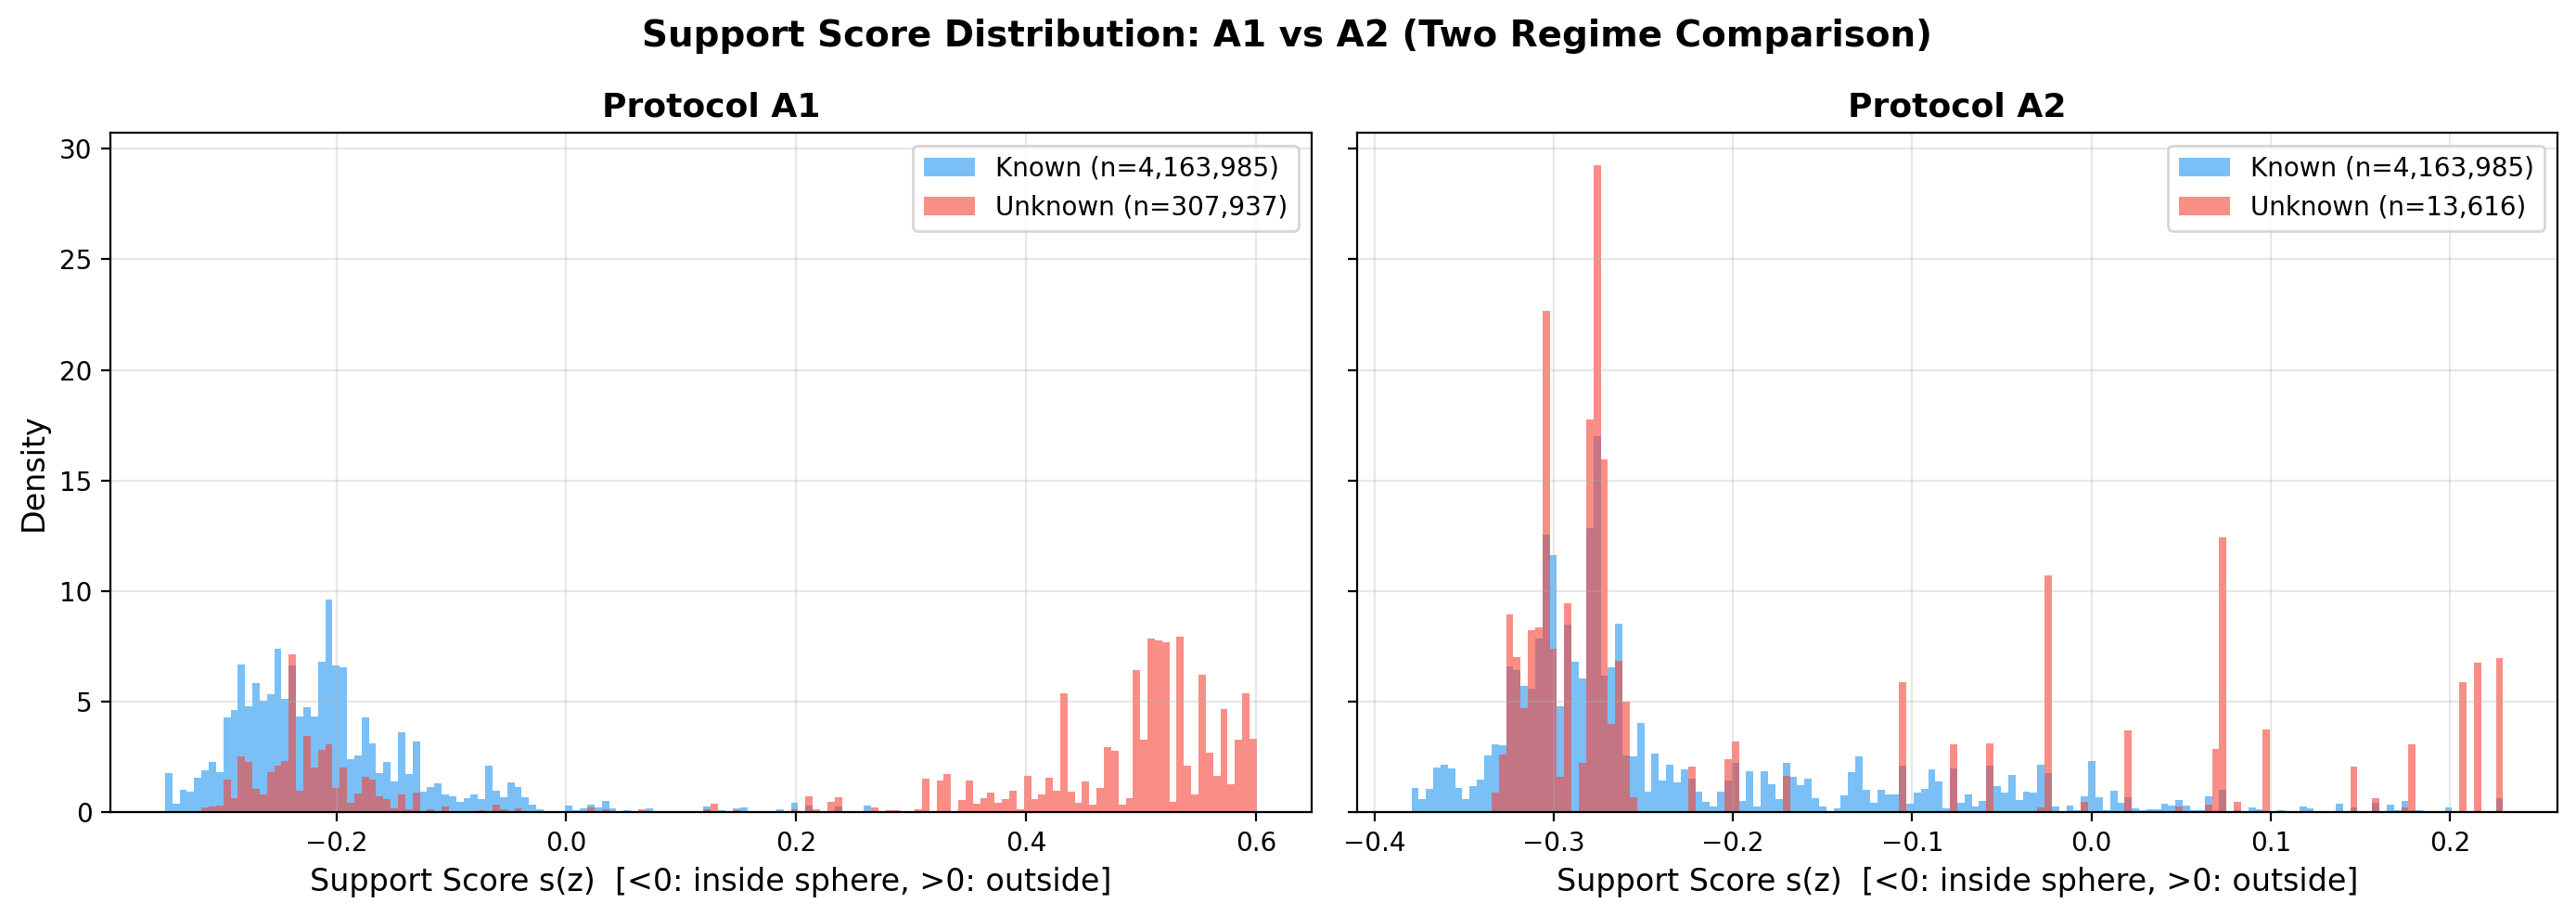
\includegraphics[width=\textwidth]{t1_support_a1_vs_a2.pdf}%
  }{%
    \IfFileExists{t1_support_a1_vs_a2.png}{%
      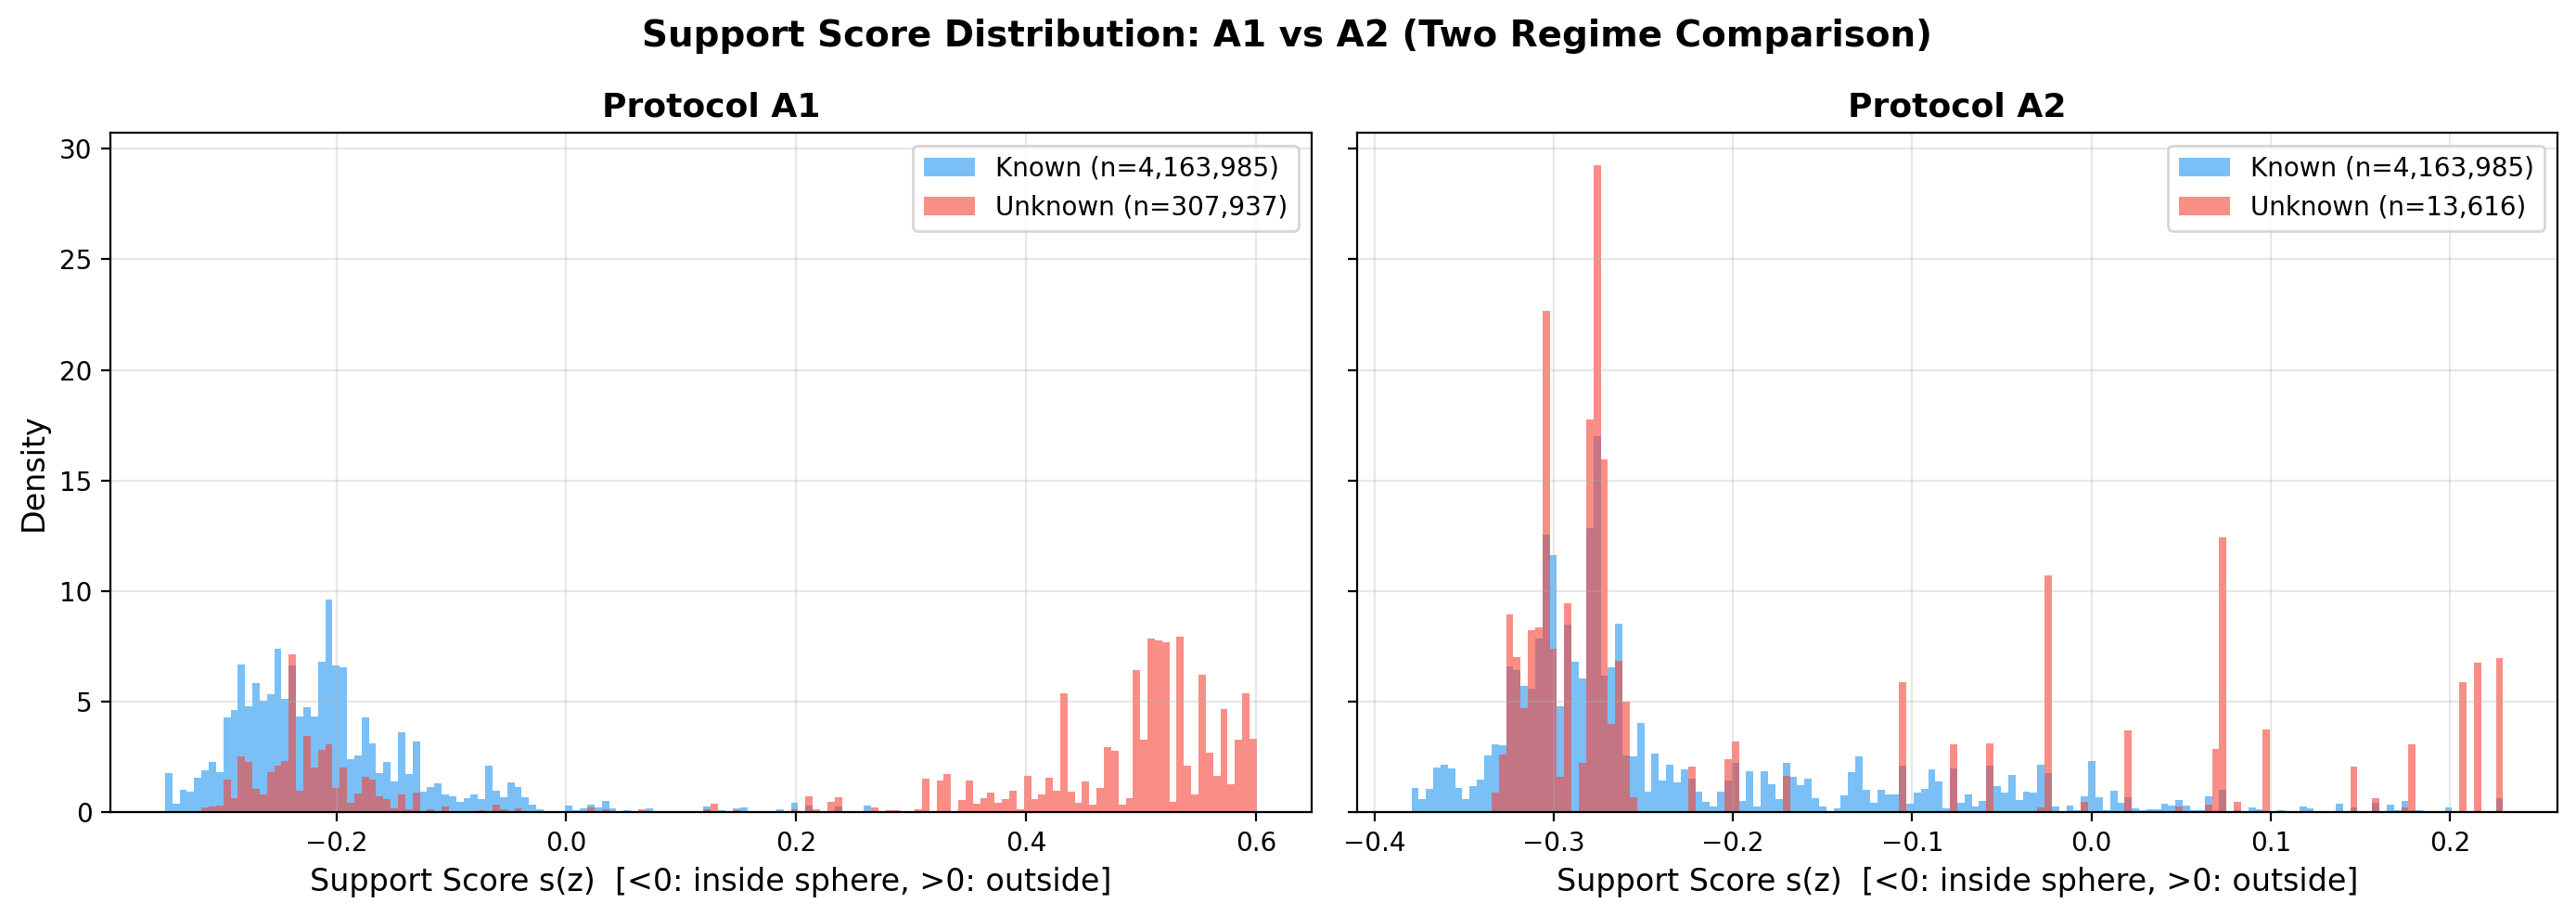
\includegraphics[width=\textwidth]{t1_support_a1_vs_a2.png}%
    }{%
      \fbox{\parbox{\textwidth}{\centering\vspace{3cm}Support score distribution comparison placeholder\vspace{3cm}}}%
    }%
  }
  \caption{Distribution comparison of support scores for known and unknown classes under A1 (left) and A2 (right). In A1, the support score distributions of known and unknown regions are clearly separated (support-deficit regime), whereas in A2 they overlap substantially (competitive-ambiguity regime), explaining why the support score's ranking capability is limited in A2.}\label{fig:score_dist}
\end{figure*}

In A1 (support-deficit regime), the support scores of unknown regions are substantially
higher than those of known regions, and the two distributions separate clearly, enabling
the support score to effectively discriminate between them.
In A2 (competitive-ambiguity regime), the support score distributions of unseen unknowns
and known classes overlap substantially, because unseen unknowns are visually similar to
certain known classes in the feature space, causing their embeddings to fall near or even
inside known-class prototype spheres, rendering the support score ineffective.
This distributional evidence intuitively explains why A2 requires switching to
classification uncertainty signals (Table~\ref{tab:a2_main}), and also validates the
necessity of the dual-protocol split---the two unknown regimes are dominated by
fundamentally different signals.

\subsubsection{A2 Retrieval Analysis}\label{sec:exp:analysis:retrieval}

Section~\ref{sec:exp:a2} observed that A2 Ensemble AUROC is high yet F1 is near zero.
To understand this phenomenon, Table~\ref{tab:retrieval} analyzes the A2 ensemble
ranking quality from a retrieval perspective.
Among foreground pixels in A2, the unknown prevalence is only 0.32\%.

\begin{table}[t]
\centering
\caption{Synapse A2 top-$r$\% retrieval analysis (ranked by ensemble score).
Lift denotes enrichment factor relative to a random baseline.}\label{tab:retrieval}
\begin{tabular}{lcccc}
\toprule
Budget & Precision & Recall & FPR & Lift \\
\midrule
top-0.1\% & $0.100$ & $0.031$ & $0.001$ & $30.8\times$ \\
top-0.3\% & $0.209$ & $0.193$ & $0.002$ & $64.3\times$ \\
top-0.5\% & $0.201$ & $0.310$ & $0.004$ & $62.0\times$ \\
top-1.0\% & $0.123$ & $0.380$ & $0.009$ & $38.0\times$ \\
\bottomrule
\end{tabular}
\end{table}

The results demonstrate that ensemble ranking has a significant enrichment effect
relative to a random baseline (lift=$64.3\times$ at top-0.3\%), but even at top-1\%,
recall is only 0.380 and precision is only 0.123.
This indicates that A2 detection signals carry clear retrieval value, but this ranking
capability is \textbf{not yet sufficient} to directly translate into high-quality
structured abstention masks.

\subsubsection{A2 Region-Level Candidate Analysis}\label{sec:exp:analysis:region}

To further diagnose the bottleneck of A2 structured abstention failure, we conduct
a region-level analysis of the candidate regions generated by unknown queries.
Across 50 slices containing unseen unknowns in A2:

\begin{itemize}[nosep]
  \item 66\% of unknown-containing slices have at least one candidate region that
        overlaps with the ground truth;
  \item However, the unknown-slice hit rate at IoU$\geq$0.10 is only 2\%;
  \item For larger connected components ($\geq$32 pixels), the hit rate at
        IoU$\geq$0.10 is 0\%;
  \item Candidate regions have 253,365 total pixels, while ground-truth unknown
        regions have only 13,616 pixels total; the candidate union IoU mean is only 0.005.
\end{itemize}

These results reveal the true bottleneck of A2 structured abstention:
\textbf{the problem lies not in the final decision step, but in candidate generation
itself.}
Although unknown queries produce coarse responses in A2, the generated candidate regions
have almost no meaningful spatial alignment with the ground truth
(union IoU$=$0.005, IoU$\geq$0.10 near zero).
Consequently, even a perfect region-level classifier cannot recover effective unknown
masks from these candidates.
This finding shifts the structuring bottleneck in A2 from ``how to make decisions''
to the more fundamental ``how to generate clean candidates,''
pointing the way for future research.


\subsection{Exploration of Candidate Purity Bottleneck Mitigation}\label{sec:exp:explore}

The analysis in Section~\ref{sec:exp:analysis} reveals that the fundamental bottleneck
of A2 structured abstention lies in candidate generation itself, not in the decision stage.
To further precisely characterize the nature of this bottleneck, we conducted exploratory
experiments along two independent pathways.

\textbf{Pathway 1: Known-Exclusion Loss.}
An intuitive hypothesis is that the invasion of unknown candidate regions into known-class
areas is the primary cause of low purity, and thus can be mitigated by explicitly
penalizing unknown responses activated within high-confidence known-class regions.
However, offline diagnosis reveals that 92.7\% of candidate pixels fall in background
regions; known interior accounts for only 27.0\% of known-class false positives,
while low-confidence foreground is the largest false-positive source (57.8\%).
This indicates that the design assumption of the exclusion loss does not match the
actual false-positive distribution.
Training validation further confirms that the optimal checkpoint for the exclusion loss
stops at epoch 1, candidate purity shows no improvement, and known-class segmentation
performance degrades.
The fundamental reason for this pathway's failure is misaligned targeting, not
insufficient loss strength.

\textbf{Pathway 2: Proposal-Conditioned Refinement.}
The second pathway constructs proposals from an ensemble anomaly map and identifies
the specific bottleneck of A2 structuring through progressive elimination.
First, offline analysis confirms that the detection signal itself is not the bottleneck:
taking the top-0.3\% pixels in the foreground and extracting connected components yields
ensemble proposal union IoU (0.153) and slice hit rate ($\text{hit@IoU}{\geq}0.10=0.70$)
far superior to the current unknown-slot candidates (0.005 and 0.02, respectively).
Second, a linear separability experiment on proposal tokens rules out feature-space
separability as the problem: matched and unmatched proposals are strongly separable in
the feature space (linear probe AUROC$=0.991$, centroid distance$=8.95$), indicating
that the required discriminative information already exists at the representation level.
This narrows the problem to the final step: how to convert separable tokens into
pixel-level coherent masks.
The attempt at this step (Table~\ref{tab:e8}) reveals the true difficulty:
directly re-drawing masks is nearly ineffective; switching to residual local
refinement (v2) brings notable improvement, but the best variant (v3b) still
has a clear gap from the theoretical upper bound of ensemble proposals.

\begin{table}[h]
\centering
\caption{Comparison of proposal-conditioned refinement variants against the ensemble proposal upper bound (A2, Synapse).}
\label{tab:e8}
\resizebox{\columnwidth}{!}{%
\begin{tabular}{lccc}
\toprule
Variant & Union IoU & Hit@IoU$\geq$0.10 & Comp Prec@IoU$\geq$0.10 \\
\midrule
E8 v1 (direct re-drawing)         & 0.039 & 0.080 & 0.048 \\
E8 v2 (residual refinement)       & 0.071 & 0.420 & 0.169 \\
E8 v3b (best variant)             & 0.073 & 0.440 & 0.172 \\
\midrule
Ensemble proposal upper bound ($r=0.3\%$) & 0.153 & 0.700 & 0.188 \\
\bottomrule
\end{tabular}
}%
\end{table}

Through progressive elimination, the two pathways jointly pinpoint the true location
of the A2 candidate purity bottleneck.
The diagnosis from the exclusion pathway shows that the spatial source of false positives
is more distributed than expected, invalidating the assumption targeting only known
interiors; the results from the proposal pathway further narrow the bottleneck from
``whether proposal tokens are separable'' (resolved, AUROC$=0.991$) to ``how to generate
pixel-level coherent masks from separable tokens'' (still open).
This localization provides a more concrete target for future work: what is needed is
not a stronger detection signal, but a generation mechanism that can bridge
proposal-level separability to pixel-level coherent masks.


\section{Discussion}\label{sec:discussion}
The results of this paper demonstrate that unknown handling in open-world dense
segmentation involves at least two fundamentally distinct capabilities: the
seen-unknown structured representation addressed by A1, and the unseen-unknown detection
generalization addressed by A2. These are dominated by different signals and correspond
to different failure modes. In A1, the key to structured output lies in whether the model
possesses an explicit unknown output space; in A2, high-quality detection ranking signals
do not automatically translate into usable structured abstention masks. Taken together
with the cross-dataset and cross-domain results, this difference is not an incidental
Synapse artifact but a general characteristic of open-world dense segmentation, as further
confirmed by experiments on PASCAL VOC and Cityscapes spanning markedly different visual domains.

At the same time, the independent baseline results also help us more clearly delineate
the boundary of the conclusions in this paper. B1 shows that a closed-set segmenter,
even with strong known-class segmentation performance, still struggles to form spatially
coherent unknown regions relying solely on post-hoc OoD signals; however, B2 also shows
that in the A1 seen-unknown fully-supervised setting, the standard $K+1$ per-pixel
segmentation is already a very strong baseline. Therefore, this paper does not attempt
to demonstrate that query-based native unknown slots are superior to all explicit unknown
modeling approaches in the fully-supervised seen-unknown setting. More precisely, this
paper validates that, relative to purely post-hoc OoD, an explicit unknown output space
is an important prerequisite for structured abstention; and this prerequisite can be
realized through different architectural forms.

Further analysis of A2 reveals that the fundamental bottleneck of current
unseen-unknown structuring failure lies not in the final decision step but in candidate
generation itself. Although both ensemble and standard per-pixel baselines can provide
strong retrieval/ranking signals, there remains insufficient spatial alignment between
unknown candidate regions and true unknown regions, with very low candidate purity.
Future work can advance along three directions: first, designing generation mechanisms
that can bridge proposal-level feature separability to pixel-level coherent masks (the
exploratory experiments in Section~\ref{sec:exp:explore} demonstrate that this bottleneck
cannot be bypassed by lightweight modifications); second, investigating structured
abstention under partial annotation, weak supervision, or open-vocabulary conditions;
third, extending validation to additional imaging modalities (MRI, ultrasound) and
dense prediction task types (panoptic, instance segmentation), building on the
cross-domain confirmation provided by the VOC and Cityscapes experiments in this paper.

This paper has several limitations.
First, while the initial formulation is motivated by medical CT, cross-domain experiments
on PASCAL VOC and Cityscapes have confirmed the core phenomena in natural-image settings.
However, further validation on additional medical modalities (MRI, ultrasound) and
dense prediction task types (panoptic, instance segmentation) remains warranted;
the framework does not rely on CT-specific assumptions, but this broader applicability
awaits independent experimental confirmation.
Second, while the 30-case scale of Synapse is consistent with similar benchmarks in this
field~\cite{chen2021transunet,cao2022swinunet}, conclusions on a single dataset still
carry the risk of overfitting to specific scanning protocols or population distributions.
We introduce AMOS22 (300 cases, CT subset) as cross-dataset validation; all three core
conclusions (A1 structured abstention, $M=0$ collapse, A2 detection--structuring gap)
are directionally consistent across two independent datasets, partially alleviating the
above concern.
Furthermore, the validation set used for threshold selection and result reporting on
Synapse contains only 4 cases; although the 100-case AMOS22 validation set produces
consistent conclusions, validation on a larger independent test set remains warranted.
Third, regarding partition robustness, this paper additionally validates an alternative
split on Synapse (Section~\ref{sec:exp:ablation:m0}, Table~\ref{tab:alt_split}), where
the $M=0$ collapse similarly holds under the alternative split (reduction of 94.6\%);
however, systematic validation across more partition combinations and datasets is left
for future work.

\section{Conclusion}\label{sec:conclusion}
This paper addresses the problem of unknown handling in dense segmentation
by proposing the Structured Abstention Segmentation (SASeg) formulation and constructing
an A1/A2 dual-protocol evaluation framework that distinguishes seen-unknown structuring
capability from unseen-unknown detection generalization capability.
Methodologically, we present a region parsing model with native unknown slots, combined
with prototype-sphere support to model the geometric support boundaries of known classes.
Experiments on medical CT datasets (Synapse, AMOS22) demonstrate that an explicit
unknown output space is important for structured abstention relative to purely post-hoc
OoD approaches; however, in the unseen-unknown setting, high detection ranking performance
does not imply usable structured outputs, and candidate purity is the current dominant
bottleneck, with exploratory experiments further showing that this bottleneck cannot be
bypassed by lightweight constraints.
Cross-domain experiments on PASCAL VOC and Cityscapes further confirm that both the
necessity of native unknown representation and the detection--structuring gap are not
confined to medical imaging but constitute general phenomena in open-world dense
segmentation.
The primary contribution of this work lies not in proposing a detector that surpasses
all baselines across every metric, but in establishing the problem formulation and
evaluation framework for structured abstention, and in characterizing the critical
boundary between detection and structuring in open-world dense segmentation.

\bibliographystyle{elsarticle-harv}
\bibliography{references}

\end{document}
